\documentclass[conference,compsoc]{IEEEtran}
\pdfcompresslevel=0
\pdfobjcompresslevel=0


\IEEEoverridecommandlockouts %%% Added for footnote in title

\ifCLASSOPTIONcompsoc
  % IEEE Computer Society needs nocompress option
  % requires cite.sty v4.0 or later (November 2003)
  \usepackage[nocompress]{cite}
\else
  % normal IEEE
  \usepackage{cite}
\fi


\usepackage[all]{nowidow}
\usepackage{siunitx}
\usepackage{multirow}
\usepackage{amsmath}
\usepackage{booktabs}
\usepackage{tabularx}
\usepackage{array}
\usepackage{makecell} % optional (not required below)
\newcolumntype{Y}{>{\raggedright\arraybackslash}X}
\usepackage[most]{tcolorbox}
\usepackage{subcaption}
% \usepackage[hidelinks]{hyperref}
\RequirePackage{doi}
\usepackage{comment}
\usepackage{amssymb}
\usepackage{fancyhdr}
\usepackage{pifont} %dingautolist 
\usepackage{float}
% break urls
% \usepackage{breakurl}
\def\UrlBreaks{\do\/\do-\do_}

\renewcommand{\sectionautorefname}{Section}
\renewcommand{\subsectionautorefname}{Section}
\renewcommand{\subsubsectionautorefname}{Section}
\renewcommand{\appendixautorefname}{Appendix}
% For appendix references
\newcommand{\refappendix}[1]{\hyperref[#1]{Appendix~\ref*{#1}}}
\newcommand{\refethics}[1]{\hyperref[#1]{Ethical Considerations}}
\newcommand{\refopenscience}[1]{\hyperref[#1]{Open Science}}

% \renewcommand{\algorithmautorefname}{Algorithm}

% Prior work comparison table
\usepackage{graphicx}
\newcommand*\rot{\rotatebox{90}}
%Circles
\usepackage{tikz}
\newcommand{\emptypie}{%
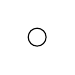
\begin{tikzpicture}
 \draw (0,0) circle (.75ex);
\end{tikzpicture}%
}
\newcommand{\pie}[1]{%
\begin{tikzpicture}
 \draw (0,0) circle (.75ex);\fill[rotate=90] (.75ex,0) arc (0:#1:.75ex) -- (0,0) -- cycle;
\end{tikzpicture}%
}
\newcommand{\xmark}{\ding{55}}%

% \usepackage{xspace}
% % Add a period to the end of an abbreviation unless there's one
% % already, then \xspace.
% \makeatletter
% \DeclareRobustCommand\onedot{\futurelet\@let@token\@onedot}
% \def\@onedot{\ifx\@let@token.\else.\null\fi\xspace}

% \def\eg{e.g\onedot}\def\Eg{E.g\onedot}
% \def\ie{i.e\onedot} \def\Ie{I.e\onedot}
% \def\cf{c.f\onedot} \def\Cf{C.f\onedot}
% \def\etc{etc\onedot} \def\vs{vs\onedot}
% \def\wrt{w.r.t\onedot} \def\dof{d.o.f\onedot}
% \def\etal{et al\onedot}
% \makeatother

\newcommand{\todo}[1]{\textcolor{red}{[#1]}}
\newcommand{\subscript}[2]{$#1 _ #2$}

\setlength{\doublerulesep}{2.5pt}

\newif{\ifanonymous}
\anonymoustrue{} % hide or show authors and other parts of the paper that should not appear at submission time


%% Gaps and Open Problem Boxed Frame
\newcommand{\gap}{\textbf{Gap}:}
\newcommand{\openproblem}{\textbf{Open Problem}:}

\usepackage[strict]{changepage}
\usepackage{framed}
\usepackage{color}

\definecolor{cosmiclatte}{rgb}{1.0, 0.97, 0.91}
\definecolor{darkred}{HTML}{AE4132}
\definecolor{lightred}{HTML}{FAD9D5}

% keywords search criteria
\newenvironment{exclusionkeywordbox}{%
  \def\FrameCommand{%
    {\color[HTML]{f8cecc}\vrule width 2pt}%
    \colorbox[HTML]{f8cecc}%
  }%
  \MakeFramed{\advance\hsize-\width\FrameRestore}%
  \noindent\hspace{-4.55pt}%
  \begin{adjustwidth}{}{7pt}%
}
{%
\end{adjustwidth}\endMakeFramed%
}

\newenvironment{keywordbox}{%
  \def\FrameCommand{%
    {\color[HTML]{d5e8d4}\vrule width 2pt}%
    \colorbox[HTML]{d5e8d4}%
  }%
  \MakeFramed{\advance\hsize-\width\FrameRestore}%
  \noindent\hspace{-4.55pt}%
  \begin{adjustwidth}{}{7pt}%
}
{%
\end{adjustwidth}\endMakeFramed%
}

% open problems
\newenvironment{opbox}{%
  \vspace{-8pt}%
  \def\FrameCommand{%
    {\color{darkred}\vrule width 2pt}%
    \colorbox{lightred}%
  }%
  \MakeFramed{\advance\hsize-\width\FrameRestore}%
  \noindent\hspace{-4.55pt}%
  \begin{adjustwidth}{}{2pt}%
  \openproblem%
}
{%
\end{adjustwidth}\endMakeFramed%
\vspace{-8pt}%
}


% gaps
\newenvironment{gapbox}{%
  \def\FrameCommand{%
    {\color{darkgray}\vrule width 2pt}%
    \colorbox{lightgray}%
  }%
  \MakeFramed{\advance\hsize-\width\FrameRestore}%
  \noindent\hspace{-4.55pt}%
  \begin{adjustwidth}{}{7pt}%
  \gap%
}
{%
\end{adjustwidth}\endMakeFramed%
}



% Defense deployment

\newcommand{\dNative}{\ding{108}} % in-browser
\newcommand{\dExt}{\ding{117}} % extension
\newcommand{\dTool}{\ding{109}} % offline/list tool
\newcommand{\dServer}{\ding{115}} % server/network/protocol/OS
\newcommand{\dNo}{\textemdash} % no/unknown industrial defense


% Tracker capabilities

% Circle fills (light pastels)
\definecolor{capIncBg}{HTML}{DBEAFE}
\definecolor{capExeBg}{HTML}{FEE2E2}
\definecolor{capObsBg}{HTML}{FEF3C7}
\definecolor{capStoBg}{HTML}{CCFBF1}
\definecolor{capShaBg}{HTML}{EDE9FE}

% Circle borders
\definecolor{capIncBd}{HTML}{93C5FD}
\definecolor{capExeBd}{HTML}{FCA5A5}
\definecolor{capObsBd}{HTML}{FCD34D}
\definecolor{capStoBd}{HTML}{5EEAD4}
\definecolor{capShaBd}{HTML}{C4B5FD}

\newcommand{\capsym}[3]{%
  \tikz[baseline=-0.55ex]{%
    \node[circle, fill=#1, draw=#2, line width=0.4pt,
          inner sep=0pt, minimum size=2.1ex,
          font=\fontsize{8}{8}\selectfont\bfseries\sffamily,
          text=black]{#3};}}

\newcommand{\symInclusion}{\capsym{capIncBg}{capIncBd}{I}}
\newcommand{\symExecution}{\capsym{capExeBg}{capExeBd}{E}}
\newcommand{\symObservation}{\capsym{capObsBg}{capObsBd}{O}}
\newcommand{\symStorage}{\capsym{capStoBg}{capStoBd}{T}}
\newcommand{\symSharing}{\capsym{capShaBg}{capShaBd}{S}}





% Icons for tracking mechanisms

\newlength{\iconsize}
\setlength{\iconsize}{0.9em}
 
\newcommand{\iconURL}{\raisebox{-0.15em}{
\includegraphics[height=\iconsize]{figures/icons/url.png}}}
\newcommand{\iconFingerprint}{\raisebox{-0.15em}{
\includegraphics[height=\iconsize]{figures/icons/fingerprint.png}}}
\newcommand{\iconCookie}{\raisebox{-0.15em}{
\includegraphics[height=\iconsize]{figures/icons/cookie.png}}}
\newcommand{\iconJS}{\raisebox{-0.15em}{
\includegraphics[height=\iconsize]{figures/icons/js.png}}}
\newcommand{\iconPrivacy}{\raisebox{-0.15em}{
\includegraphics[height=\iconsize]{figures/icons/privacy.jpg}}}
\newcommand{\iconBehavioral}{\raisebox{-0.15em}{
\includegraphics[height=\iconsize]{figures/icons/behavioral.png}}}
\newcommand{\iconSC}{\raisebox{-0.15em}{
\includegraphics[height=\iconsize]{figures/icons/sc.png}}}

\newcommand{\iconAdBlock}{\raisebox{-0.15em}{\includegraphics[height=\iconsize]{figures/icons/block.png}}}
\newcommand{\iconCNAME}{\raisebox{-0.15em}{\includegraphics[height=\iconsize]{figures/icons/cname.png}}}



\newcommand{\iconBlocklist}{\raisebox{-0.15em}{
\includegraphics[height=\iconsize]{figures/icons/blocklist.png}}}
\newcommand{\iconExtension}{\raisebox{-0.15em}{
\includegraphics[height=\iconsize]{figures/icons/extension.png}}}
\newcommand{\iconTool}{\raisebox{-0.15em}{
\includegraphics[height=\iconsize]{figures/icons/tool.png}}}



% Browser icons
\newcommand{\iconIE}{\raisebox{-0.3em}{
\includegraphics[height=1.6em]{figures/icons/ie.png}}}
\newcommand{\iconEdge}{\raisebox{-0.3em}{
\includegraphics[height=1.6em]{figures/icons/edge.png}}}
\newcommand{\iconFirefox}{\raisebox{-0.3em}{
\includegraphics[height=1.6em]{figures/icons/firefox.png}}}
\newcommand{\iconSafari}{\raisebox{-0.3em}{
\includegraphics[height=1.6em]{figures/icons/safari.png}}}
\newcommand{\iconChrome}{\raisebox{-0.3em}{
\includegraphics[height=1.6em]{figures/icons/chrome.png}}}
\newcommand{\iconBrave}{\raisebox{-0.3em}{
\includegraphics[height=1.6em]{figures/icons/brave.png}}}





% Defense Goals

% Detection and Blocking
\definecolor{cellred}{RGB}{252,235,235}
% Signal Reduction and Obfuscation
\definecolor{cellyellow}{RGB}{255,253,230}
% Regulation compliance
% Incentives
\definecolor{cellpink}{RGB}{243,230,248}
% Expectations
\definecolor{cellblue}{RGB}{230,241,253}
% Responsibilities
\definecolor{cellgreen}{RGB}{232,250,235}



\definecolor{cellempty}{RGB}{242,242,248}
\newcommand{\ec}{\cellcolor{cellempty}}
\newcommand{\rh}{\rule[-0.9em]{0pt}{2.0em}}
\newcommand{\cellsym}[1]{\parbox[c][2.0em][c]{\linewidth}{\centering #1}}




% \usepackage[landscape,margin=0.35in]{geometry}
\usepackage{calc}
\usepackage[table]{xcolor}



% TBD to create a warning at compilation (i.e., to not forget to edit later)
\newcommand{\TBD}[2]{\errmessage{#1}{[#2]}}
% \newcommand{\TBD}[1]{\errmessage{TBD}{\color{red}{[#1]}}}

%% Students
\newcommand{\yash}[1]{\textcolor{red}{[\textbf{Yash Vekaria}: #1]}}
\newcommand{\yohan}[1]{\textcolor{olive}{[\textbf{Yohan Beugin}: #1]}}
\newcommand{\shaoor}[1]{\textcolor{blue}{[\textbf{Shaoor Munir}: #1]}}

%% Professors
\newcommand{\alexandros}[1]{\textcolor{cyan}{[\textbf{AK}: #1]}}
\newcommand{\franzi}[1]{\textcolor{magenta}{[\textbf{Franziska Roesner}: #1]}}
\newcommand{\gunes}[1]{\textcolor{yellow}{[\textbf{Güneş Acar}: #1]}}
\newcommand{\jason}[1]{\textcolor{brown}{[\textbf{Jason Polakis}: #1]}}
\newcommand{\nataliia}[1]{\textcolor{cyan}{[\textbf{Nataliia Bielova}: #1]}}
\newcommand{\nick}[1]{\textcolor{green}{[\textbf{Nick Nikiforakis}: #1]}}
\newcommand{\pierre}[1]{\textcolor{orange}{[\textbf{Pierre Laperdrix}: #1]}}
\newcommand{\sebastian}[1]{\textcolor{pink}{[\textbf{Sebastian Zimmeck}: #1]}}
\newcommand{\steven}[1]{\textcolor{purple}{[\textbf{Steven Englehardt}: #1]}}
\newcommand{\umar}[1]{\textcolor{teal}{[\textbf{Umar Iqbal}: #1]}}
\newcommand{\zubair}[1]{\textcolor{violet}{[\textbf{Zubair Shafiq}: #1]}}


\newcommand{\para}[1]{\smallskip \noindent \textbf{#1}}
\newcommand{\parait}[1]{\smallskip \noindent \textit{#1}}

%Logos affiliations
\newcommand{\ucDavis}{\raisebox{2pt}{
\includegraphics[width=30pt]{figures/logos/uc-davis.pdf}}}
\newcommand{\uwMadison}{
\includegraphics[height=10pt]{figures/logos/uw-madison.pdf}}
\newcommand{\radboud}{
\includegraphics[height=10pt]{figures/logos/radboud.pdf}}
\newcommand{\inria}{
\includegraphics[height=10pt]{figures/logos/inria.pdf}}
\newcommand{\cnrs}{
\includegraphics[height=10pt]{figures/logos/cnrs.pdf}}
\newcommand{\washU}{
\includegraphics[height=10pt]{figures/logos/washU.jpg}}
\newcommand{\ncstate}{\raisebox{2pt}{
\includegraphics[width=30pt]{figures/logos/ncstate.pdf}}}
\newcommand{\stonybrook}{
\includegraphics[height=10pt]{figures/logos/stonybrook.pdf}}
\newcommand{\uic}{
\includegraphics[height=10pt]{figures/logos/uic.pdf}}
\newcommand{\uwashington}{
\includegraphics[height=8pt]{figures/logos/uwashington.pdf}}
\newcommand{\wu}{
\includegraphics[height=10pt]{figures/logos/wu.pdf}}
\newcommand{\independent}{\raisebox{2pt}{$\dagger$}}
\usepackage{xurl} % break long urls

% correct bad hyphenation here
% \hyphenation{op-tical net-works semi-conduc-tor}

% Squeeze space on paragraphs
\renewcommand{\paragraph}[1]{\vspace{0.1in}\noindent\textbf{#1}}

\anonymousfalse{}


\begin{document}
%
% paper title
% Titles are generally capitalized except for words such as a, an, and, as,
% at, but, by, for, in, nor, of, on, or, the, to and up, which are usually
% not capitalized unless they are the first or last word of the title.
% Linebreaks \\ can be used within to get better formatting as desired.
% Do not put math or special symbols in the title.
\title{\LARGE{\textbf{SoK: Advances and Open Problems in Web Tracking}}\thanks{\textbf{An extended and living version of this document is available at \url{https://github.com/privacysandstorm/sok-advances-open-problems-web-tracking}}}}



% author names and affiliations
% use a multiple column layout for up to three different
% affiliations
\ifanonymous
\author{\em Anonymous Authors}
\else
\author{
    \IEEEauthorblockN{
        Yash Vekaria\IEEEauthorrefmark{1}~\ucDavis{}, 
        Yohan Beugin\IEEEauthorrefmark{1}~\uwMadison{}, 
        Shaoor Munir~\ucDavis{}, 
        Gunes Acar~\radboud{}, 
        Nataliia Bielova~\inria{}, \\
        Steven Englehardt~\independent{}, 
        Umar Iqbal~\washU{},
        Alexandros Kapravelos~\ncstate{},   
        Pierre Laperdrix~\cnrs{},
        Nick Nikiforakis~\stonybrook{},\\ 
        Jason Polakis~\uic{},
        Franziska Roesner~\uwashington{},
        Zubair Shafiq~\ucDavis{}, 
        Sebastian Zimmeck~\wu{}
    }
    \IEEEauthorblockA{\ucDavis{}~University of California, Davis, USA}
    \IEEEauthorblockA{\uwMadison{}~University of Wisconsin–Madison, USA}
    \IEEEauthorblockA{\radboud{}~Radboud University, Netherlands}
    \IEEEauthorblockA{\inria{}~Inria Centre at Université Côte d’Azur, France}
    \IEEEauthorblockA{\independent{}~Independent Researcher, USA}
    \IEEEauthorblockA{\washU{}~Washington University in St. Louis, USA}
    \IEEEauthorblockA{\ncstate{}~North Carolina State University, USA}
    \IEEEauthorblockA{\cnrs{}~Centre National de la Recherche Scientifique (CNRS), France}
    \IEEEauthorblockA{\stonybrook{}~Stony Brook University, USA}
    \IEEEauthorblockA{\uic{}~University of Illinois Chicago, USA}
    \IEEEauthorblockA{\uwashington{}~University of Washington, USA}
    \IEEEauthorblockA{\wu{}~Wesleyan University, USA}
}

\fi

% make the title area
\maketitle

\begingroup\renewcommand\thefootnote{\IEEEauthorrefmark{1}}
\footnotetext{Equal contribution.}
\endgroup

%%%% Page number and header bar
\pagestyle{fancy}
\fancyhf{}
\fancyfoot[C]{\thepage}
\setcounter{page}{1}



% no keywords

%-------------------------------------------------------------------------------
\input{short-version/0-abstract}
%%
\section{Introduction}
\label{sec:introduction}

%%
Users access a variety of free content and services on the web, which are largely funded through online advertising.
%
In turn, advertising is heavily dependent on monitoring users' online activities for various purposes 
%
such as analytics, (re)targeting, and conversion tracking.
%
To realize these objectives, user tracking has become a pervasive part of the web.
%
% Online advertising in the US alone is set to exceed \$400 billion in 2025~\cite{adSpendEmarketer2025}.

%%
Ever since the introduction of cookies on the web in the mid-1990s, web tracking has evolved into a significantly more prevalent and sophisticated practice.
%
Around 92\% of webpages today embed at least one third-party tracker~\cite{urban2024WebAlmanac2024}.
%
Moreover, user tracking and profiling often involves collection of user's personal details (\eg{}, name, email, and location), device characteristics (\eg{}, device model and operating system), browsing history, and behavioral signals (\eg{}, time spent on a page and performed interactions).
%
As a result, web tracking has become an active area in online privacy research.

%%
Over the years, researchers have conducted numerous studies to examine the evolution of web tracking mechanisms, browser developments, and regulatory compliance. 
%
Most survey papers have either been too high-level~\cite{ermakova2018web} or too narrowly-focused on specific forms of web tracking such as caching and browser fingerprinting~\cite{bujlowSurveyWebTracking2017, laperdrix2020browser}. 
%
Overall, despite a considerable body of work, major findings remain scattered across many disparate studies.
%%
Furthermore, as privacy defenses improve in browsers, trackers continually adapt with new evasion techniques~\cite{narayanan2018web, localmess-usenix-sec-26}.
%
The result is an ever-shifting technical landscape of tracking techniques.
%
Regulations often govern tracking practices and ensure that browsers provide necessary protections to safeguard user privacy.
%
Although these regulatory changes have had a more gradual impact than browser-based technical interventions, together they have continued to reshape the ecosystem. 
%
Today, web tracking is undergoing a transformative change due to the introduction of privacy-enhancing protections in major web browsers and evolving regulatory frameworks.
%
% Recent advancements in online advertising comprise the introduction of privacy-preserving paradigms and adoption of generative AI on the web~\cite{builtin-ai,chavezUpdatePlansPrivacy2025}.
At the same time, advertising paradigms that do not rely on cross-site tracking have been introduced, and are being standardized at the W3C~\cite{chavezUpdatePlansPrivacy2025, hercherW3CAdPrivacy2022}.
%
% In light of these shifts, it is important and timely to 
These shifts call for a comprehensive and systematic study of emerging trends in the evolving tracking landscape to identify crucial research gaps.
%
% Thus, the research community can clearly benefit from a unified resource that consolidates and systematizes the state of knowledge, helping researchers to make meaningful contributions to the field and ensure a structured approach at addressing new privacy issues.

%%
To this end, in this SoK, we synthesize the disparate lines of research and practices in web tracking---spanning across technical mechanisms, browser mitigations, as well as regulatory changes---to systematically provide an overview of the current state of web tracking. 
%
We scope this work to how the data is \textit{collected} about users, not how that data might then be \textit{used}. 
%
This unified perspective enables a critical reflection on how far the community has come and which research directions it should prioritize.
% in terms of research directions.
%
Our contributions are: % as follows:
%
\begin{itemize}
    \item We systematically organize the extensive body of research on web tracking, providing a consolidated knowledge base of advances in the field, highlighting evolving trends, bridging emerging but related tracking mechanisms and identifying gaps in the field.
    % \vspace{-2.5mm}
    \item We provide an overview of major browser-based anti-tracking interventions and relevant regulatory frameworks across the EU and the US to assess how they have altered the ecosystem over the years.
    % \vspace{-2.5mm}
    \item We identify key open challenges and promising future directions in the domain of web tracking for the community to address in the coming years.
\end{itemize}
%%
\section{Methodology}
\label{sec:methodology}

Online tracking has a vast literature, comprising numerous research studies published over the last few decades.
%
As a result, we first carry out a literature survey to identify all papers related to web tracking published in the last 20 years (2005 onward) at any of the seven top web security and privacy venues---IEEE S\&P, USENIX Security, ACM CCS, NDSS, ACM IMC, PETS, and WWW.
%
A total of 200+ research papers were identified. 
%
Each paper was assigned one or more topics related to web tracking based on their abstract. 
% \footnote{The thematic organization is available at \url{https://osf.io/zsy7e/overview?view_only=a346b98bf89244b5b17d842f6fb3fb13}}.
%
The assignment of topics was jointly performed by two researchers following Clarke and Braun’s thematic analysis approach~\cite{clarke2013successful}.
%
A total of 40 topical themes were identified (see \autoref{sec:thematic-analysis}), with the top 15 (by number of papers) being tracking measurements, tracking in browsers and mobile, browser fingerprinting, regulation compliance, profiling, third-party tracking, cookie consent, cookies, user studies in tracking, ad blocking, JavaScript-based tracking, side-channels, advertising and tracking defenses, and browser extension fingerprinting.
%
We used our domain expertise to structure the SoK around these prominent themes as outlined in the rest of this paper. 


%  We extracted all papers published in the last 20 years (2005 onward) at any of the following top web security, privacy, and measurement venues—IEEE S&P, USENIX Security, ACM CCS, NDSS, ACM IMC, PETS, and WWW. Then, two researchers filtered these papers by agreeing on their relevance to web tracking based on their titles and abstracts, and assigned to included papers one or more topics, following Clarke and Braun’s thematic analysis approach [39]. A total of 200+ papers and 40 themes were identified. The SoK was primarily structured around the identified papers and completed as needed with any relevant literature from other venues based on our domain expertise. [...]’’
\input{short-version/3-background}
%%
% \vspace{-2mm}
\section{Threat Model of Web Tracking}
\label{sec:threat-model}
% \vspace{-1mm}

%%
Our threat model for web tracking considers four main entities: user, browser, first-party website, and third-parties included in the website. 
%
The user is an individual accessing websites on the internet through their browser (also known as user agent~\cite{mdnUserAgentMDN2025}), seeking to keep their online behavior private. % and hence considered the \textit{victim}. % or at least under control. 
%
Browsers mediate all interactions between the user and the web content, enforcing the different policies described in~\autoref{sec:background}. % and providing necessary functionality for webpages. 
%
The first-party website is a webpage that the user directly visits to browse content. 
%
It often includes resources from third-parties that are not directly visited by the user and are typically hosted on a different domain than the first-party website~\cite{mdnDomainMDNWeb2024}.
%
A tracker is any party whose goal is to collect data about the user’s activities in order to profile or identify the user’s behavior across the web. % across one (\textit{same-site tracking}) or more sites (\textit{cross-site tracking}) or across devices (\textit{cross-device tracking}). 
%
We consider first- and third-party trackers as \textit{adversaries}, where their aim is to gather maximum information on users. %consistent with their capabilities.
%
\autoref{fig:threat-model} provides a conceptual overview of our model where \texttt{news.com} and \texttt{sports.com} are the first-party websites visited by the user from their personal device(s). 
%
\texttt{tracker1.com} and \texttt{tracker2.com} are the third-parties embedded on the first-party websites.



\begin{figure}
    \centering
    
\includegraphics[width=\linewidth]{figures/threat-model.pdf}
    \caption{Threat model of web tracking.}
    \label{fig:threat-model}
    % \vspace{-5mm}
\end{figure}



%%
\para{Adversary Goals.} 
%
% The primary goal of an adversary is to identify and correlate user data across the web for purposes such as profiling, analytics, or ad targeting.
%
User data can be divided into two categories: (1) identifiers such as email, or identifying information such as network, software, or hardware configurations, and (2) browsing activity comprising webpages visited and website interactions performed by the user. 
%
The tracker's goal can be distinguished into different scopes:
%
\textbf{\textit{Same-site}.} 
The tracker aims to profile or identify a returning user on the same first-party website across multiple visits or page loads. 
%
\textbf{\textit{Cross-site}.} 
%
Trackers embedded on multiple unrelated first-party websites often aim to profile or identify a user across these sites in order to link different website activities to the same user.
%
\textbf{\textit{Cross-device}.} 
%
A tracker may also aim to profile or identify the same user as they browse the internet using different devices or browsers. 
%
% For instance, \texttt{tracker1.com} embedded on \texttt{news.com} would like to know that the user \texttt{X} on a mobile phone is the same as user \texttt{Y} browsing the same website a little later from a desktop device.
%
In summary, the adversary's primary goal is to persistently and uniquely label the user or the user’s browser/device and to collect user data tied to that label, across navigations, sites, and over time, for purposes such as profiling, analytics, or ad targeting.
%
Besides, a secondary goal of the tracker may be to avoid detection or prevention; \ie{}, achieving their goal despite anti-tracking measures.


%%
\para{Adversary Capabilities.} 
%
% A tracker's capabilities are shaped by the web's architecture and browser's security model discussed in ~\autoref{sec:background}.
%
To achieve their goals, an adversary's capabilities can be explained in context of \textit{inclusion}, \textit{collection}, \textit{storage}, and \textit{sharing} of the user data, subject to the browser's context-origin restrictions discussed in~\autoref{sec:background}.
%
The adversary is considered capable enough to track users either in presence of these browser-enforced policy restrictions or by circumventing them.
%
\textbf{\textit{Inclusion}.} 
%
A first-party tracker is assumed to directly monitor user activities within the top-level browsing context.
%
A third-party tracker could be embedded as an inline resource (\eg{}, image/script tag) within the mainframe by the first-party assuming trust delegation, an iframe with a separate context under its origin (\ie{}, with its own DOM, state, and resources), or as a resource within a third-party iframe, isolated from the mainframe context. 
%
% By including an executable resource (\eg{}, script) on the webpage, tracker gains the ability to run code in the user’s browser, subject to script execution context requirements governed by browser's context model discussed in~\autoref{sec:background}.
% %
% With an embedded non-executable resource (\eg{}, image), a tracker can still initiate resource loading requests to its server, sharing cookies along with the request.
% %
% We assume the tracker could use one or more inclusion methods described above depending on what the first-party allows.
%
\textbf{\textit{Collection}.}
%
A tracker aims to collect user data through available browser features by either executing JavaScript code or reading browser storage.
%
\textbf{\textit{Storage}.}
%
Trackers may read, write, or modify data in the user's browser using \texttt{localStorage}, \texttt{sessionStorage}, \texttt{indexedDB}, and the cookie jar.
%
The stored data can be accessed by the tracker in subsequent visits to either the same site or a different site.
%
\textbf{\textit{Sharing}.}
%
To share the collected user data with its own servers or a partner's tracking server, trackers can initiate network requests including the user data in one of four ways: (1)~as a request URL query parameter, (2)~request payload, (3)~request header, or (4)~through HTTP cookies.
%
Approaches 1-3 require tracking scripts to explicitly include user data, whereas HTTP cookies associated with the tracker's domain are automatically included in all requests to the tracker's server. % (\eg{}, setting a custom request header for tracking).
%
% In case of 4, browsers automatically attach the previously set tracker's cookies with the requests sent to the tracker’s domain as a request header, even if that request originates in a first-party context. 
%%
% We use this threat model to understand different web tracking mechanisms and their evolution over time.



%%
\section{Stateful Tracking}
\label{sec:stateful-tracking}
%%
The most straightforward approach to tracking a user involves storing a unique identifier in their browser and retrieving it or modifying it as they browse different websites, which is a process known as ``stateful tracking''. 
%
Browsers provide a number of interfaces (e.g., cookies, see \autoref{tab:appendix-stateful-tracking}) that are designed to associate \textit{state} to the user's visit, and others that store information as a side effect of some other functionality provided to the website (e.g., E-Tags, HSTS upgrades), which trackers can sometimes abuse to encode a unique identifier~\cite{englehardtAutomatedDiscoveryPrivacy2018,ashkansoltaniFlashCookiesPrivacy2011,solomosTalesFaviconsCaches2021}.
%
% \noindent The capabilities of a tracker %depends on the restrictions 
% are governed by browsers security model defined in \autoref{sec:background}: (1) script execution privileges (2) context of inclusion (3) storage access policies.




%%
\subsection{Third-party Stateful Tracking}
\label{sec:tp-stateful}

\para{Cookies.} Cookies---first specified by Lou Montulli at Netscape in 1990s---allow maintaining a state when the browser communicates with a web server via HTTP, a stateless protocol~\cite{kristolHTTPCookiesStandards2001}. 
%
For example, a website can store a user’s authentication token in the browser via a cookie, which is then shared with the web server with each request that the user’s browser makes, allowing the website to verify the user’s authentication status. 
%
Browsers mediate which resources and domains are able to access specific cookies~\cite{beugin2024WebAlmanac2024,singhIncoherenciesWebBrowser2010,mdnSameoriginPolicySecurity2024}.

\begin{figure}[htbp]
    \centering
    
\includegraphics[width=1\linewidth]{figures/tracking-mechanisms-cookie.pdf}
    \caption{Cookie-based Tracking.}
    \label{subfig:cookie-tracking}
\end{figure}

%%
First- or third-party domains on a webpage can set and receive cookies through either \texttt{cookie} and \texttt{set-cookie} headers in network requests and responses respectively or via the \texttt{document.cookie} or CookieStore JavaScript API.
%
Cookies set in a first-party context on a website are called first-party cookies, allowing a user to be re-identified to the website that they visit. 
%
Similarly cookies set in a third-party context are classified as third-party cookies and they allow cross-site tracking. 
%
For example, in \autoref{subfig:cookie-tracking}, \texttt{news.com} and \texttt{sports.com} both include iframes with ads from \texttt{tracker.com}. 
%
As a result, the user’s browser will send the same \texttt{tracker.com} cookie with requests to load the iframes on both pages. 
%
On \texttt{tracker.com} server's side, these two requests can be attributed to the same user and combined with additional information about the user-visited website. 
% (from the HTTP Referrer header or query parameters passed along when the request to load the iframe is made). 
%
Privacy concerns with third-party cookies were identified as early as their introduction~\cite{montulliHTTPStateManagement1997,kristolHTTPCookiesStandards2001} as public concern over web tracking grew.
% elevated to the point where the FTC held a workshop on the topic in 1997. 
% and the United States government banned and audited the use of cookies on government websites~\cite{SenatorRaisesPrivacy2001}. Nonetheless, this mechanism 
Nonetheless, cookies have been the dominant form of web tracking for many years. 

%%

\para{Cookie Syncing.}
%%
Third-parties included on a few websites, are only able to track users across that limited number of sites~\cite{roesnerDetectingDefendingThirdparty2012,lernerInternetJonesRaiders2016}. 
%
Moreover, under the SOP restriction, a third-party on a webpage cannot share its cookies with another third-party domain by directly initiating a request to it.
%
To overcome these constraints and exchange information collected about the user on different websites, third-party companies rely on cookie syncing or cookie matching~\cite{acarWebNeverForgets2014}---first described by Olejnik et al.~\cite{olejnikSellingPrivacyAuction2014} and also named as ``referred tracking'' by Roesner et al.~\cite{roesnerDetectingDefendingThirdparty2012}. 
%
Earlier works formalized cookie syncing detection approach~\cite{acarWebNeverForgets2014,englehardtOnlineTracking1millionsite2016,bashirTracingInformationFlows2016}, that has been further improved~\cite{papadopoulosCookieSynchronizationEverything2019} and used to build sophisticated ML-based detection approaches~\cite{papadopoulosCookieSynchronizationEverything2019, iqbalKhaleesiBreakerAdvertising2022}.

\begin{figure}[htbp]
    \centering
    
\includegraphics[width=1\linewidth]{figures/tracking-mechanisms-cookie-syncing.pdf}
    \caption{Cookie Syncing.}
    \label{subfig:cookie-syncing}
\end{figure}

%%
This mechanism relies on synchronizing user identifiers known to two different third parties that are typically stored in third-party cookies and most commonly shared via URL parameters. 
%
% Following from the previous example, let’s suppose there are 
If amongst two trackers (\texttt{tracker1.com} and \texttt{tracker2.com}), only \texttt{tracker1.com} is present on \texttt{news.com} as shown in \autoref{subfig:cookie-syncing}, it can share its user identifier stored in a third-party cookie by initiating a request to \texttt{tracker2.com} and adding it in the URL parameter. 
%
This would allow \texttt{tracker2.com} to know the identifier the user has for \texttt{tracker1.com}, match it with the user identifier of \texttt{tracker2.com}, and communicate server-to-server to further merge the information collected about this user by \texttt{tracker1.com} and \texttt{tracker2.com}. 


%%

\para{Tracking Tags.}
%%
Traditionally, tracking pixels (or invisible pixels) used to be 1x1 image elements embedded on a webpage that pointed to some tracking endpoint~\cite{Narayanan2017WebtapSpringer,englehardtOnlineTracking1millionsite2016}.
%
When a user visits a webpage embedding a 1x1 pixel, user data is shared with the tracker, allowing user tracking on the same site as well as cross-site.
%
Image-based tracking pixels have been primarily used for analytics, ad (re)targeting, and conversion tracking. 
%
Researchers have conducted various large-scale measurements to study image-based tracking pixels \cite{lernerInternetJonesRaiders2016,agarwal2021under,vekaria2021differential}.

\begin{figure}[htbp]
    \centering
    
\includegraphics[width=1\linewidth]{figures/tracking-mechanisms-tracking-tags.pdf}
    \caption{Tracking Scripts.}
    \label{subfig:tracking-scripts}
\end{figure}

%%
Over the years, the capabilities of tracking pixels have significantly advanced.
%
Modern tracking pixels, also referred to as tracking tags, rely on JavaScript to collect finer-grained information in browsers~\cite{bekosHitchhikersGuideFacebook2023}. 
%
\autoref{subfig:tracking-scripts} represents a simple scenario where a tracking pixel from \texttt{tracker.com} is embedded on the homepage as well as on the \texttt{/signup} page of \texttt{news.com}, respectively collecting and sharing button clicks and form events with its own server, with the help of its tracking script.
%
Thus, tracking pixels have expanded in scope to support additional use cases, such as managing multiple pixels via a single tag, bot detection, and session replays~\cite{senolLeakyFormsStudy2022,acarNoBoundariesData2020,englehardtNoBoundariesCredentials2018}.




%%
\subsection{First-party Stateful Tracking}
\label{sec:fp-stateful}


%%
Since most browsers either block \cite{TrackingPreventionWebKit2020} or partition third-party access (by origin) to stateful APIs \cite{mdnThirdpartyCookiesPrivacy2024}, trackers aren’t able to store and retrieve identifiers \textit{across} sites. 
%
At best, storage partitioning allows tracking user activity on a single site.
%
To circumvent these protections, trackers adopt first-party based mechanisms described in this section.

%%

\para{Cookies.}
\label{subsubsec:stateful-tracking-cookies}
%%
When third-party tracking scripts are embedded into first-party execution contexts, the scripts execute with the same privileges as first-party scripts, allowing them to read and write JavaScript-accessible first-party storage as if they were a first-party script~\cite{bahramiCOOKIEGUARDCharacterizingIsolating2024}. 
%
First-party cookies often store unique user identifiers created with browser fingerprinting and those which are bounced through navigational tracking (see~\autoref{subfig:navigational-tracking}). 
%
Recent research \cite{munirCookieGraphUnderstandingDetecting2023,vekaria2024WebAlmanac2024} has shown that nearly 90\% of all websites use at least one tracking first-party cookie, 96\% of which are in fact set by third-party scripts running in a first-party context.
%%
% 
Additionally, research has shown that it is difficult to get rid of these tracking cookies.
%
Once a user clears their cookies, the tracker can use information stored elsewhere on the web browser to ``respawn'' or reconstruct the user’s identifier, creating a so-called ``supercookie'' or ``evercookie''~\cite{ayensonFlashCookiesPrivacy2011,soltaniFlashCookiesPrivacy2009,fouadMyCookiePhoenix2022} as described in \autoref{sec:stateful-defenses-evercookie}.

\para{Cookie Syncing.}
%%
One of the privacy issues with first-party cookies is syncing these identifiers with other third-parties. 
%
This sharing---first described by Fouad et al.~\cite{fouadMissedFilterLists2020}---allows third-parties to collude and benefit from information gathered across different websites in a first-party context. 
%
In some cases, first-party cookies set by Google and Facebook are shared with hundreds of other third-party domains~\cite{munirCookieGraphUnderstandingDetecting2023,bahramiCOOKIEGUARDCharacterizingIsolating2024}.
%
% In addition to syncing first-party cookies, trackers also combine personal information obtained from users across different websites to create extensive identity graphs of users as described in~\autoref{sec:id-providers} to track users in absence of third-party cookies.


%%

\para{Tracking Tags.}
%%
Blocking third-party cookies renders tracking pixels embedded as image elements ineffective. 
%
However, modern tracking tags that rely on JavaScript can still be used to track users in a first-party context~\cite{munirCookieGraphUnderstandingDetecting2023}. 
%
These tags are often included in the main frame context of a website by the developer, allowing pixel tracking companies to monitor different user activities using first-party execution privileges.


%%

\para{Navigational Tracking.}
% \label{sec:navigational-tracking}
%%
A popular mechanism for sharing identifiers is via link decorations as depicted in \autoref{subfig:navigational-tracking}. 
%
Recent research has identified query parameters, resource paths, and URL fragments being used for sharing user data, such as first-party cookies and email addresses, on more than 70\% of websites~\cite{munirPURLSafeEffective2024}, in absence of third-party cookies or first-party partitioning. 
%
Besides link decorations, bounce tracking is another navigation-based mechanism that allows trackers to read/write their cookies across sites, rendering third-party cookie blocking ineffective~\cite{kellyBounceTrackingMitigations2022}. 


\begin{figure}[htbp]
    \centering
    
\includegraphics[width=1\linewidth]{figures/tracking-mechanisms-navigational-tracking.pdf}
    \caption{Navigational Tracking.}
    \label{subfig:navigational-tracking}
\end{figure}

%%
At a high level, a tracker’s goal is to momentarily surface or visit its own domain in the browser’s \emph{first-party} context, because this lets it read and write identifiers that persist in first-party storage. 
%
\autoref{subfig:bounce-tracking} shows a typical \textbf{bounce-tracking} sequence:
%
\ding{182} a third-party script on \texttt{news.com} reads first-party identifier(s) stored under \texttt{news.com} and
%
\ding{183} includes them in the request to \texttt{tracker.com}.
%
\ding{184} Browser redirects to \texttt{tracker.com}, either by a user click, automatically (e.g., \texttt{window.location.href="...";}, or a \texttt{<meta http-equiv="refresh">}).
%
\ding{185} Once loaded as a \emph{first party}, \texttt{tracker.com} reads the identifier from the URL or merges it with an existing cookie, rewriting the URL to its final destination (e.g., back to \texttt{news.com} or other domain), embedding the consolidated identifier.
%
\ding{186} The browser navigates to \texttt{news.com}; the tracker’s script there extracts the identifier from the decorated URL and 
%
\ding{187} stores it in \texttt{news.com}’s first-party storage, completing the cross-context or cross-site linkage if redirected to same first-party or a different domain.

\begin{comment}
% \begin{enumerate}[label=(\roman*)]
\begin{dingautolist}{182}
  \item A third-party script on \texttt{news.com} reads any first-party identifier already stored under \texttt{news.com}.
  \item Identifier is included in the request to \texttt{tracker.com}.
  \item Browser redirects—either by a user click or automatically (e.g., \texttt{window.location.href="...";} or a \texttt{<meta http-equiv="refresh">})—to \texttt{tracker.com}.
  \item Once loaded as a \emph{first party}, \texttt{tracker.com} reads the identifier from the URL or merges it with an existing cookie, rewriting the URL to its final destination (e.g., \texttt{sports.com}), embedding the consolidated identifier.
  \item Browser navigates on to \texttt{sports.com}; the tracker’s script there extracts identifier from the decorated URL and stores it in \texttt{sports.com}’s first-party storage, completing the cross-site linkage.
\end{dingautolist}
\end{comment}

\begin{figure}[htbp]
    
    \centering
    
\includegraphics[width=1\linewidth]{figures/tracking-mechanisms-bounce-tracking.pdf}
    \caption{Bounce Tracking.}
    \label{subfig:bounce-tracking}
\end{figure}

Bounce chains can involve two sites (\texttt{news.com} → \texttt{tracker.com} → \texttt{news.com}) or longer, allowing the tracker to propagate a stable user identifier across multiple unrelated websites despite third-party cookie restrictions.
%
% As a result of this process, a tracker is able to use the same identifier across websites. 
%
Due to potential usability disruptions and the implementation of defensive measures, bounce tracking is not widely pervasive
\cite{iqbalKhaleesiBreakerAdvertising2022}.
%
Measurements in 2020 found that 11.6\% of sites use one of the top 100 redirectors~\cite{koopInDepthEvaluationRedirect2020}, and in 2022 such identifiers were present in 8.1\% of crawled navigations~\cite{randallMeasuringUIDSmuggling2022}.


%%
\subsection{Defenses Against Stateful Tracking}
\label{sec:stateful-defenses}


Given the broad adoption of stateful tracking and its perceived intrusive nature, numerous tracking countermeasures have been proposed by the research community; some have been adopted by browsers, others are available through extensions.

%%

\subsubsection{Third-party Stateful Tracking Protections}
\label{sec:stateful-defenses-evercookie}
%%
\para{Clearing Cookies.}
Logically, a user could clear the cookies in their browser at the end of each session to protect themselves from being tracked. 
%
However, browser cookie clearing features do not typically clear \textit{all} stateful mechanisms provided to sites \cite{acarWebNeverForgets2014, englehardtOnlineTracking1millionsite2016}. 
%
For example, clearing cookies often does not remove identifiers stored in browser storage APIs \texttt{localStorage}~\cite{ayensonFlashCookiesPrivacy2011,roesnerDetectingDefendingThirdparty2012}, \texttt{IndexedDB}~\cite{acarFPDetectiveDustingWeb2013}, E-Tags~\cite{ayensonFlashCookiesPrivacy2011}, and browser cache~\cite{sorensenZombiecookiesCaseStudies2013}. 
%
A malicious tracker can take advantage of this limitation by storing copies of their tracking identifiers in locations that aren’t cleared by the browser. 
%
The most publicized example of such cookies (or "supercookies") was Adobe's Flash browser plugin, which provided no mechanism for browsers to clear its storage \cite{soltaniFlashCookiesPrivacy2009,solomosTalesFaviconsCaches2021}.
%
Any API that allows a tracker to persist state to the user’s device is a potential supercookie vector~\cite{aliNavigatingMurkyWaters2023}. 
%
% Even just a single bit of storage can be abused if a tracker is able to string together multiple calls to an API, each encoding another bit from the identifier.
%
Kamkar first demonstrated how widespread this risk is by encoding identifiers in APIs like HTTP Strict Transport Security (HSTS), Web Cache, \texttt{window.name}, and Web History~\cite{kamkarSamyKamkarEvercookie2010}. 
%
Variants of the same attack were also demonstrated later on with other browser APIs~\cite{klink1334485TrackingUsing2017,goodinUnpatchedBrowserWeaknesses2015,evansPublicKeyPinning2015}. 
%
Ultimately supercookie risk was the prime motivation behind the network and storage partitioning efforts of Firefox, Chrome, and Safari~\cite{menkeStorageIsolationProject2020,privacycommunitygroupClientSideStoragePartitioning2022,mdnStatePartitioningPrivacy2024}. 
%
As of 2025, most browsers have blocked/partitioned third-party access to stateful APIs, preventing their use for cross-site tracking.

%%
\para{Restrictions on Third-party Cookies.}
%
Browsers attempt to block most third-party cookies~\cite{mdnThirdpartyCookiesPrivacy2024} but exceptions exist to support non-tracking use cases such as enabling single sign-on (SSO), whose removal may lead to website breakage \cite{crouchImprovingPrivacyBreaking2018}. 
%
Privacy-focused browsers, such as Brave, apply the most aggressive restrictions by blocking all third-party cookies by default and allowing third-parties to share a partitioned ephemeral storage for the lifetime of the session \cite{braveprivacyteamEphemeralThirdpartySite2021}. 
% (i.e., until the browser is closed or the last instance of first-party website (eTLD+1) closes)~\cite{braveprivacyteamEphemeralThirdpartySite2021}.
%
Among the mainstream browsers, Safari and Firefox have the most effective restrictions. 
%
Safari currently blocks all third-party cookies unless the domain (eTLD+1) has been visited by the user as a first-party or if the third-party explicitly requests to use the cookies through the Storage Access API~\cite{TrackingPreventionWebKit2020}. 
%
It further relies on an ML model to detect whether the domains with third-party access engage in tracking and restrict their cookies if the user has not interacted with them as a first-party in the last 30 days. 
%
Firefox blocks third-party cookies from known trackers (as determined by the Disconnect tracking protection list~\footnote{\url{https://disconnect.me/trackerprotection}}) and also partitions third-party cookies, such that each first-party and third-party origin combination has a separate cookie jar~\cite{mdnThirdpartyCookiesPrivacy2024}.
%
Initially, following in the footsteps of Safari and Firefox, Google Chrome announced plans to block all third-party cookies~\cite{chromeBuildingMorePrivate2020}, which after several delays, it decided not to proceed with~\cite{chavezNewPathPrivacy2024}. 
%
Chrome currently offers various tools for developers to manage third-party cookies, including JavaScript APIs like the Storage Access API~\cite{mdnStorageAccessAPI2024} and cookie directives like the ``SameSite' attribute~\cite{mdnSetCookieHTTPMDN2024}. 
%
However, trackers may not adhere to or use these mechanisms.
%
Moreover, trackers have also migrated to alternative tracking techniques by circumventing existing protections.
%
%
Hence, researchers~\cite{panNotKnowWhat2015} have also proposed a tracking-free web browser that isolates identifiers into a different browser principal so that they exist but are not unique across different websites, thereby severing the third-party tracking chain.


\para{Blocking Trackers.}
%%
Filter lists are widely used by browsers (e.g., Brave) and browser extensions (e.g., uBlock Origin) to block third-party tracking requests.
%
However, filter list based ad or tracker blocking faces significant limitations: 
%
(1) manually curated lists are maintained by small community individuals and do not capture nuanced techniques, 
%
(2) as lists grow in size, they contain outdated or too narrow entries (e.g., 90\% of EasyList rules are practically never triggered~\cite{snyderWhoFiltersFilters2020}),
%
(3) being static, trackers keep evading them.
%
To overcome these challenges, researchers have focused on building ML-driven advertising or tracking request blockers ~\cite{iqbalAdGraphGraphBasedApproach2020, sibyWebGraphCapturingAdvertising2022, yangWTAGRAPHWebTracking2022, leAutoFRAutomatedFilter2023}.
%
AutoFR \cite{leAutoFRAutomatedFilter2023} proposes a fully automated framework for filter rule creation and evaluation.
%
While AdGraph \cite{iqbalAdGraphGraphBasedApproach2020}, WebGraph \cite{sibyWebGraphCapturingAdvertising2022}, and WTAGraph \cite{yangWTAGRAPHWebTracking2022} treat a webpage as a graph of HTML structure, network requests, and JavaScript behavior, to train a classifier for identifying and subsequently blocking advertising and tracking resources.
%
These approaches can generalize sufficiently to discover previously unknown trackers and adapt to evolving tracking behaviors. 
%
Brave implements an AdGraph-based ML solution (PageGraph) to detect and block trackers.
%
Beyond network requests and CNAME-based blocking~\cite{daoCNAMECloakingBasedTracking2021}, another popular anti-tracking method is to detect and block tracking scripts or JavaScript code at different granularities~\cite{ikramSeamlessTrackingFreeWeb2017,smithSugarCoatProgrammaticallyGenerating2021} such as domain-based and path-based script blocking~\cite{leCVInspectorAutomatingDetection2021,alrizahErrorsMisunderstandingsAttacks2019,snyderWhoFiltersFilters2020}, function-level blocking~\cite{amjadBlockingJavaScriptBreaking2023,amjadBlockingTrackingJavaScript2024} or event loop based blocking~\cite{chenDetectingFilterList2021} within an otherwise benign script \cite{amjadTrackerSiftUntanglingMixed2021}. %
Adversarial trackers are incentivized to evade such blocking (e.g., by changing script location or causing site breakage), thus posing challenges.


%%

\subsubsection{Protections Against First-party Circumventions}

\para{Restrictions on First-party Cookies.}
Unlike third-party cookies, first-party cookies cannot be as easily blocked completely because it would break critical website functionality such as maintaining login state. 
%
Therefore, they require more targeted countermeasures as listed below. 

%%
\para{Limiting Lifetime of First-party Storage Written by Tracking Scripts.}
%
Safari’s Intelligent Tracking Protection (ITP) expires all first-party cookies or storage set by scripts after no user interaction for 7 days \cite{TrackingPreventionWebKit2020}. 
%
To mitigate workarounds that automatically overwrite cookies written by scripts with HTTP cookies, Safari detects third-party hosts cloaked under first-party subdomains using heuristics applied to the first-party host’s CNAME and IP address~\cite{TrackingPreventionWebKit2020}. 
%
Brave implements a limited version of this, which caps the lifetime of cookies set by scripts to 7 days~\cite{bravePrivacyProtectionSecurity}.

%%
\para{Removing or Limiting the Persistence of Identifiers Passed in URL Parameters.}
%
Several browsers remove URL parameters known to be used by trackers. 
%
Firefox~\cite{mozillaQueryParameterStripping} implements removal in a non-default mode, while Brave~\cite{braveprivacyteamGrabBagQuery2020} and DuckDuckGo~\cite{duckduckgoDuckDuckGoWebTracking} ship it by default. 
%
When URL parameters are removed on navigation, embedded tracking scripts are prevented from accessing tracking IDs across sites. 
%
Safari takes a different approach: instead of removing tracking parameters, it limits the lifetime of script-accessible storage from 7 days to 24 hours when ITP detects link decoration~\cite{TrackingPreventionWebKit2020}.



%%
\para{Limiting First-party Storage Set During a Bounce.}
%
Bounce tracking not only circumvents third-party storage protections but also allows unrestricted access to tracker’s first-party storage. 
%
Browsers mitigate it by differentiating between a \textit{legitimate visit} to a site and a brief \textit{bounce} for tracking purposes. 
%
The fact that some authentication flows appear similar to bounce tracking complicates this issue~\cite{kellyBounceTrackingMitigations2022}. 
%
Brave and Firefox use blocklists to detect potential bounce trackers, whereas Safari and Chrome use heuristics based on site behavior as mitigations~\cite{snyderNavigationalTrackingMitigations2024}. 
%
Firefox, Chrome, and Safari delete all site storage for these domains unless there's evidence of legitimate and recent user interaction with the site; the definition of \textit{legitimate} and \textit{recent} varies by browser~\cite{snyderNavigationalTrackingMitigations2024,TrackingPreventionWebKit2020}. 
%
While Brave provides suspected bounce trackers with access to ephemeral storage that is cleared once all tabs opened from that tracker are closed, so long as the tracker does not already have persistent storage set~\cite{braveprivacyteamUnlinkableBouncingMore2022}.


%%\
\para{Blocking First-party Cookies.}
Privacy-enhancing extensions support targeted deletion of known tracking cookies, including first-party cookies, through a filter list \cite{ublockResourcesLibrary,adguardrteamScriptletsWikiAboutscriptletsmd,schininaSourceBehavioralCookieremoverjs2024}.
%
While filter lists face the aforementioned challenges, they can also be automatically curated using an ML-based approach \cite{munirCookieGraphUnderstandingDetecting2023,bollingerAutomatingCookieConsent2022,schoniBlockCookiesNot2024a}.
\section{Stateless Tracking}
\label{sec:stateless-tracking}

Under stateless tracking (see \autoref{tab:appendix-stateless-tracking}), trackers do not rely on a stored state (\ie{}, ID) in the browser to track a user, and instead collect artifacts of the user's behavior, browser, or hardware to generate a fingerprint to correlate a user across sites and sessions.
% 
Analysis of real-world fingerprints and entropy computations have revealed that some attributes can contribute a lot more to the uniqueness of users than others, leading to the identification of a specific user with high certainty~\cite{eckersleyHowUniqueYour2010,laperdrixBeautyBeastDiverting2016,gomez-boixHidingCrowdAnalysis2018,bacis2024assessing}. 
%
% \autoref{tab:appendix-stateless-tracking} summarizes different mechanisms and defenses.


%%
\subsection{Fingerprinting and Types}

Fingerprinting corresponds to the gathering of information on users’ behavior, browsers, and devices in real-time with the goal of identifying users. 
%
\autoref{fig:stateless-tracking} depicts how fingerprinting works; through HTTP headers and calls to specific JavaScript APIs, a website can collect a wide range of information on the user's behavior (\eg{} mouse movements, keystrokes, and clicking), browser (\eg{} browser version, screen size, installed fonts, GPU model, timezone and preferred languages), and configuration of the underlying OS and the hardware. 
% 
Its use for tracking purposes has been hard to detect and block, as fingerprinting can be used (1) constructively, to identify user-impersonating actors such as bots or fraudsters, and (2) destructively to identify and track users who wish to remain anonymous (see~\autoref{sec:need-for-fingerprinting}). 
%
Additionally, it is difficult to prevent as users exhibit the same behavior and retain the same device over time, which can result in certain stable fingerprinting attributes.
%
Several types of fingerprinting techniques exist based on the nature of the collected attributes.
% Among them, browser fingerprinting has been the most studied and widely used mechanism in context of the web. 

\begin{figure}[htbp]
    \centering
    
\includegraphics[width=0.85\linewidth]{figures/tracking-mechanisms-fingerprinting.pdf}
    \caption{Stateless Tracking via Fingerprinting.}
    \label{fig:stateless-tracking}
\end{figure}

%%
\para{Browser Fingerprinting.} 
%
Relying on browser-based APIs to collect information about configurations of the browser, device or the underlying OS to generate a fingerprint is referred to as browser fingerprinting.
%
Since the first academic work on browser fingerprinting in 2009~\cite{mayerAnyPersonPamphleteer2009}, researchers have studied: its impact on privacy~\cite{eckersleyHowUniqueYour2010}, its use with other tracking techniques~\cite{fouadMyCookiePhoenix2022} and in real world applications~\cite{aminazadWebRunner20492020, wuHimManyFaces2023}, its detection~\cite{iqbalFingerprintingFingerprintersLearning2021, boussahaFPtracerFinegrainedBrowser2024}, abusable browser APIs~\cite{bahramiFPRadarLongitudinalMeasurement2022, suAutomaticDiscoveryEmerging2023, senolDoubleEdgedSword2024}, and user protections~\cite{vastelFpScannerPrivacyImplications2018}. 
%
The Electronic Frontier Foundation’s Panopticlick project \cite{effpanopticlick} provided one of the earliest large-scale empirical demonstrations of browser fingerprintability and associated risks. 
% and has been influential in characterizing real-world browser fingerprinting risks.
%
In 2013, fingerprinting was observed on $\sim$1\% of the top 10K websites~\cite{nikiforakisCookielessMonsterExploring2013} and $\sim$400 of the top 1M websites~\cite{acarFPDetectiveDustingWeb2013}. 
%
Over the years, a variety of techniques have been used to measure browser fingerprinting~\cite{acarWebNeverForgets2014,englehardtOnlineTracking1millionsite2016,olejnikBatteryStatusNot2017,dasWebsSixthSense2018}, with two general trends being: its higher adoption by third-parties and its expansion to a diverse set of browser APIs over the years. 
%
By 2021, fingerprinting scripts were found to be present on 10\% of the top 100K websites, with more popular ones having a higher incidence (\ie{}, 30\% of the top 1,000)~\cite{iqbalFingerprintingFingerprintersLearning2021}.
%
Importantly, browser fingerprints are not always stable enough to track users over time: 80\% of browser instances change fingerprints in less than 10 days~\cite{vastelFPSTALKERTrackingBrowser2018}. 
%
Trackers not only link fingerprints as they evolve, but also combine and persist them with \textit{stateful} techniques, rendering the technique effective even in browsers that partition third-party access to stateful APIs (\autoref{sec:stateful-defenses}). 
%
A 2022 study measured a lower bound on this approach by detecting cookie respawning due to browser fingerprinting on 1,150 of the top 30K sites~\cite{fouadMyCookiePhoenix2022}.
%
Prior works have explored various browser-supported JavaScript APIs for fingerprinting such as Canvas~\cite{moweryPixelPerfectFingerprinting2012}, WebGL~\cite{caoCrossBrowserFingerprintingOS2017}, Audio API~\cite{englehardtOnlineTracking1millionsite2016}, the Battery Status API~\cite{olejnikLeakingBatteryPrivacy2016}, as well as font and device-class characteristics exposed through rendering and system metrics~\cite{fifield2015fingerprinting,bursztein2016picasso}.
%
Other recent works indicate that fingerprinting risks differ across demographics~\cite{berkeHowUniqueWhose2025} and that certain information contained in fingerprints could be limited without breaking the user experience~\cite{intumwayaseUARadarExploringImpact2023}.\\



%%
\para{Side-channel Fingerprinting.} 
% 
% Trackers may also exploit available browser APIs and resources to find new side-channels to fingerprint the user's browser or device. 
% %
% Besides browser fingerprinting techniques, researchers have demonstrated numerous side-channel approaches to track users.
%
Side-channel fingerprinting research has evolved from early demonstrations of unintended browser state leakage—such as history sniffing~\cite{weinbergStillKnowWhat2011}, cache abuse~\cite{shusterman2021prime+}, and favicon-based persistence~\cite{solomosTalesFaviconsCaches2021}—to increasingly systematic and automated analyses of cross-site information flows in modern browsers~\cite{knittelXSinatorcomFormalModel2021}. 
%
As defenses have closed individual leaks, subsequent work has shifted towards identifying newer classes of tracking vectors, leveraging timing~\cite{jinTimingBasedBrowsingPrivacy2022}, resource contention~\cite{snyderPoolPartyExploitingBrowser2023}, and feature exposure~\cite{aliNavigatingMurkyWaters2023} as more subtle fingerprintable signals within the browser. 
%
More recently, side-channel techniques have expanded beyond the browser’s internal state to external observables such as network metadata~\cite{leeNettrackGenericWeb2023} and physical signals~\cite{jeonImListeningYour2018}, enabling coarse tracking even under strong isolation or encryption assumptions. 
%
Together, this line of work has suggested a trajectory away from brittle single-mechanism attacks and toward compositional and cross-layer side channels that exploit performance optimizations, shared infrastructure, and user interactions. 
%
Generally, side-channel attacks are challenging to detect and could be equally difficult to mitigate.

%%
\para{Extension Fingerprinting.} 
%
This other side-channel approach aims at inferring the presence of specific extensions in user's browser~\cite{karamiCarnusExploringPrivacy2020}. 
%
Early studies~\cite{sjostenDiscoveringBrowserExtensions2017, gulyasExtendNotExtend2018, karamiCarnusExploringPrivacy2020} demonstrated how extensions contain specific resources (\eg{},~images, scripts) that can be referenced by web pages, thereby revealing their presence. 
%
Researchers have also explored behavioral extension fingerprinting~\cite{starovXHOUNDQuantifyingFingerprintability2017, karamiCarnusExploringPrivacy2020, solomosDangersHumanTouch2022, solomosEscapingConfinesTime2022, laperdrixFingerprintingStyleDetecting2021, agarwalPeekingWindowFingerprinting2024}, where an extension can be implicitly inferred through executional side-effects, and corresponding mitigations~\cite{karamiUnleashSimulacrumShifting2022, sanchez-rolaExtensionBreakdownSecurity2017} such as randomizing WARs, IDs, or classes~\cite{trickelEveryoneDifferentClientside2019}, and access control based extension loading~\cite{sjostenLatexGlovesProtecting2019}. 


%%
\para{Behavioral Fingerprinting.} 
%
% Behavioral fingerprinting involves using browser APIs and setting-up event listeners to record user's behavior (\eg{} mouse movements, keystrokes, click behavior, and other interaction patterns) on a website, that are known to be unique for a given user~\cite{leivaMyMouseMy2021}.
%
Early work on behavioral fingerprinting has shown that fine-grained interaction signals such as mouse movements can reliably distinguish users and support continuous or implicit authentication~\cite{zhengEfficientUserVerification2011,jorgensenMouseDynamicsBehavioral2011}, even in realistic adversarial settings~\cite{fereidooniAuthentiSenseScalableBehavioral2023}. 
%
Similarly, keystroke patterns from user's typing behavior can be used to reliably link a user across their devices~\cite{yuanCrossdeviceTrackingIdentification2018}.
%
Such behavioral signals are commonly used in bot detection and inference of user attributes from interaction traces~\cite{leivaMyMouseMy2021}. 


%%
\para{Hardware Fingerprinting.} 
%
Sanchez-Rola et al. demonstrated how JavaScript APIs can be used to construct a hardware fingerprint by analyzing the execution timing of instruction sequences~\cite{sanchez-rolaClockClockTimeBased2018}, while others have demonstrated browser-based fingerprinting techniques that target the device's CPU~\cite{trampertBrowserBasedCPUFingerprinting2022,matyuninTrackingPrivateBrowsing2018} or GPU~\cite{laorDRAWNAPARTDevice2022}. 
%
Recent research also demonstrates DRAM-based device fingerprinting capabilities from the vantage point of browsers~\cite{venugopalanFPRowhammerDRAMBasedDevice2024}.
%
Hardware-related fingerprints have also been extensively explored within the mobile ecosystem~\cite{bojinovMobileDeviceIdentification2014,dasTrackingMobileWeb2016,marcantoniLargescaleStudyRisks2019,hupperichRobustnessMobileDevice2015,deyAccelPrintImperfectionsAccelerometers2014,zhang2019sensorid}, due to the availability of additional sensors (\eg{}, gyroscope, magnetometer) which can exhibit unique hardware ``imperfections'' that occur during the manufacturing process. 
%
%
More broadly, any browser mechanism that extracts some form of data or affects client-side policies or behavior without storing a user-specific identifier, should be treated as a potential stateless tracking vector and analyzed accordingly~\cite{aliNavigatingMurkyWaters2023}. 

%%
\subsection{Defenses Against Stateless Tracking}
\label{sec:stateless-defenses}

%%
Browser vendors consider fingerprinting as a form of covert tracking harmful to the web~\cite{nottinghamUnsanctionedWebTracking2015}. 
%
Major browsers have deployed some fingerprinting mitigation and the W3C encourages specification authors to consider how their APIs contribute to the browser fingerprinting surface~\cite{dotyMitigatingBrowserFingerprinting2019}. 
%
Despite this, browsers continue to expose a significant amount of fingerprintable information.
%
No optimal strategy exists as it often comes at the cost of user's utility. 
%
There is rather a disagreement on the feasibility of entirely mitigating fingerprinting and the value of deploying incremental improvements without a clear path to complete mitigation~\cite{snyderBraveFingerprintingPrivacy2019,rescorlaTechnicalCommentsPrivacy2021}. 
%
% As such, fingerprinting mitigations vary greatly across browsers.

\para{Normalization.}
%%
Normalization of device information exposed by browsers is the most common approach to reduce the utility of fingerprints. 
%
Liu et al.~\cite{liuGummyBrowsersTargeted2022} proposed spoofing of a wide variety of attributes to mimic other browsers to defend against fingerprinting.
%
This is similar to browsers such as Tor that make fingerprints consistent across users, thereby making it hard to differentiate between them~\cite{perryDesignImplementationTor2013}. 
%
Browsers have reduced identifying information exposed by APIs already shipped to the web (freezing the minor browser version from the User-Agent string~\cite{weissIntentDeprecateFreeze2020} and deploying User-Agent reduction~\cite{davisReleaseNotesSafari2017,kimura1609304ReduceGeckos2020,googleWhatUserAgentReduction2024}), removed web APIs known to be abused for fingerprinting (unshipping the Battery Status API~\cite{olejnikBatteryStatusNot2017}), and declined to implement new APIs that expose additional fingerprinting surfaces (WebKit and Firefox’s refusal to adopt the Network Information API~\cite{TrackingPreventionWebKit2020,thomsonNetworkInformationAPI2018}). 

\para{Randomization.}
%
Web API normalization sometimes breaks websites that expect to have access to device information. 
%
% For example, Mozilla rolled back their effort to freeze the Android OS version in Firefox for Android’s User-Agent string due to breakage on a major authentication provider~\cite{peterson1865766FreezeAndroid2024}. 
%
For these web APIs, browsers have added site-specific randomized noise to the outputs of the APIs, for example, noise added to the rasterized outputs of the 2D Canvas, to WebGL renderings, and \texttt{AudioBuffer} samples from the WebAudio API. 
%
Randomization was first deployed by Brave under the name ``farbling’’~\cite{braveprivacyteamFingerprintingDefenses202020}, and was later adopted by Firefox~\cite{huang1816056FprandomizationMeta2023} and Safari~\cite{wilanderPrivateBrowsing202024}. It causes a single user's fingerprint to keep changing from page load to page load, complicating user tracking. 
%
These latter countermeasures are easier to deploy across user populations and hence more popular than the ones which aim to make all environments appear identical\cite{nikiforakisPriVaricatorDeceivingFingerprinters2015}.
% 
Crucially though, alternative fingerprinting techniques can still be employed~\cite{linFashionFauxPas2023} and trackers can adapt their collection strategies in response to deployed defenses~\cite{vastel2020fp}.

\para{Anti-fingerprinting Policies.}
%%
Besides changes to individual API outputs, browsers have also explored approaches grounded in policy to discourage fingerprinting. 
%
Mozilla released an anti-tracking policy which forbids fingerprinting~\cite{mozillaSecurityTrackingPolicy2019} and subsequently blocked scripts from loading in Firefox when they were detected to include code doing so~\cite{englehardtFirefox72Blocks2020}. 
%
Such runtime blocking of fingerprinting scripts using static and dynamic analysis based automated detection often fail under obfuscation tactics~\cite{faizkhademi2015fpguard}.
% 
%
Google Chrome engineers proposed the \textit{Privacy Budget} scheme, where websites would be allowed to access device information up to a browser-defined budget~\cite{lasseyMikewestPrivacybudget2019}.
%
Once that budget is exceeded, the browser would limit further exposure of identifying information. 
%
This approach was met with skepticism due to a likelihood of website breakage and risk of exposing additional tracking surface~\cite{snyderBraveFingerprintingPrivacy2019, rescorlaTechnicalCommentsPrivacy2021}, resulting in its discontinuation~\cite{leflerWhatHappenedPrivacy2024}. 
%

Overall, a lack of unified effort in the last decade suggests how challenging it can be to tackle fingerprinting.

% Thus, a lack of unified effort in the past decade to tackle fingerprinting suggests that, as of now, there is no desire in the tech community to remove it entirely. 
%%
\section{Cross-device Tracking}
\label{sec:cross-device}

\para{Types of Cross-device Tracking.} Cross-device tracking can be \textit{deterministic} or \textit{probabilistic}. Traditionally, user’s account information such as username or email addresses have been used to link or associate browsing activity across devices~\cite{kimProbabilisticVisitorStitching2017,cottaOffPolicyEvaluationProbabilistic2019,brookmanCrossDeviceTrackingMeasurement2017}. When these deterministic identifiers fail, for example, if the user is logged out, probabilistic signals are used such as (a) IP addresses shared by multiple devices belonging to the same user~\cite{diaz-moralesCrossDeviceTrackingMatching2015}, (b) URL browsing patterns~\cite{phanCrossDeviceMatching2017}, (c) OS and hardware characteristics~\cite{caoCrossBrowserFingerprintingOS2017}, or (d) user behavior such as typing~\cite{yuanCrossdeviceTrackingIdentification2018}. These features are combined by trackers into \textit{cross-device graphs}~\cite{zimmeckPrivacyAnalysisCrossdevice2017,wangGraphTrackGraphbasedCrossDevice2022}.

\para{Limitations.} However, probabilistic techniques do not always provide a reliable identifier (e.g., ISPs dynamically rotate and share public IP addresses across several households). As a result, trackers employ proprietary algorithms to eliminate noise, such as ignoring commercial, private, and proxied IP ranges from cross-device graph computations, or setting fine temporal thresholds for observed identifiers to be considered originating from the same user.


\para{Defenses Against Cross-device Tracking.} Users logged in on the same account on different devices inherently limit the effectiveness of deterministic cross-device protections. On the other hand, probabilistic cross-device protections are, principally, the same as against traditional tracking, e.g., limiting the disclosure of user data that could be used to correlate users. 
On mobile devices, techniques have been introduced to intercept, inspect, and block outgoing packets from apps~\cite{shubaNoMoAdsEffectiveEfficient2018}. With respect to the use of inaudible ultrasound signals, efforts have pushed for the standardization of beacons and OS-level APIs to better control access to the functionality and selectively suppress certain frequencies~\cite{mavroudisPrivacySecurityUltrasound2017}.


\input{short-version/8-privacy-regulation}
%%
\section{Discussion \& Future Outlook}
\label{sec:future-outlook}

\subsection{Stateful Tracking}
\para{Shift to First-party Cookies \& Cookie Partitioning.}
Nearly half of the top most visited websites already use first-party tracking cookies. We expect this trend to continue with further adoption of third-party tracking restrictions, content-blocking tools, and partitioning.
%
Cookie partitioning is a method by which cookies are siloed or ``partitioned’’ according to the context in which they are set, effectively restricting browser-based storage to remain strictly tied to each visited site, making it more difficult to link user identities and behaviors across different sites.
%
Moreover, third-parties embedded in first-party context are able to set, access, and modify first-party data stored by other origins in absence of any origin-based partitioning~\cite{bahramiCOOKIEGUARDCharacterizingIsolating2024}.
%
Thus, partitioning is simply one aspect of a broader set of needed privacy measures: trackers can still use fingerprinting and first-party scripts in first-party context. %embedded on individual domains.

%%
\begin{opbox}
In a world without cookies, what alternative forms of user tracking are emerging that could increase privacy risks, and how might these risks manifest---for example, in light of Chrome’s recent decision not to deprecate third-party cookies anymore?
\end{opbox}


\para{More Reliance on First-party Data \& Identity Graphs.}
\label{sec:id-providers}
As restrictions are being put in place for third-party cookies, websites now lean on a handful of major \emph{identity providers} (\eg{}, Google and Meta) who, through their position as gatekeepers, can authenticate users while quietly attaching persistent, service-specific identifiers. 
%
Many platforms further fuse this stream with in-house ``first-party’’, and offline data such as loyalty-card and point-of-sale data, constructing proprietary \emph{identity graphs} that map a single user (or household) to multiple browsers, apps, and physical transactions.
%
While these integrations help publishers measure conversions and personalize content under tighter browser policies, they also concentrate behavioral insights to a few dominant actors and erode users’ ability to maintain separate or pseudonymous personas, raising fresh antitrust and privacy challenges~\cite{TargetedAdvertisingAutorite2025,khanAmazonsAntitrustParadox2017,munirGooglesChromeAntitrust2024}.
%

\begin{opbox}
How can we detect or infer opaque first-party data flows within the identity provider ecosystem, which enables persistent user tracking across devices, and quantify its privacy risks?
% How can we detect or infer opaque server-side data flows, reveal what information is shared server-side, and quantify its privacy risks?
\end{opbox}

\para{Tracking Tags.}
%%
A tag from a given pixel tracking company can be configured in many ways depending on the distinct user behaviors websites want to track. As a result, detecting the mere presence of tracking pixels is not enough.
%
It is crucial to detect all JavaScript-based tracking tags embedded on a website and study their tracking configurations to truly understand the tracking capabilities of such tags.
%%
\begin{opbox}
How are tracking tags configured differently on sites, and how does it impact tracking behavior?
\end{opbox}


% \para{Session Replays.}
% Session replay (or recording) scripts capture detailed user interactions such as keystrokes, mouse, and scrolling movements, along with the full content of the visited pages.
% %
% This allows publishers to record and playback visits as if they are ``looking over [visitors’] shoulders’’, for purposes including marketing, analytics, and troubleshooting~\cite{AdvancedUsageInspectlet}.
% %
% However, these scripts can also capture sensitive personal data filled out by visitors~\cite{acarNoBoundariesData2020,senolLeakyFormsStudy2022,yuGotSickTracked2022}, while redaction measures offered by session replay vendors are often fragile and limited in effectiveness~\cite{englehardtNoBoundariesCredentials2018,acarNoBoundariesData2020}.

\subsection{Stateless Tracking}

\para{Paywalls to Force Users to Remain Recognizable.}
To avoid limitations imposed by ad blockers~\cite{koreacopyrightcommissionNumberAdblockUsers2024}, some websites use paywalls or registration walls that require user authentication (and often payment information) before granting content access.
%
This tactic may reduce users' motivation to block cookies or browse privately, and it also requires users to remain ``recognizable’’, giving website operators a reliable identifier that persists across sessions and is more robust than third-party cookies.
%
While paywalls may support legitimate revenue models---especially for publishers facing declining ad revenues---they also create an environment where anonymity is traded for access.
%
Consequently, if paywalls become more pervasive, it may be hard for privacy-conscious users to avoid sharing their personal data online.

%%
\begin{opbox}
How do publishers leverage paywalls to build first-party profiles, and how do they associate authenticated users with online behaviors (\eg{}, shopping) to enable targeted advertising within their own networks?
\end{opbox}


\para{Server to Server Data Sharing}
%
To circumvent ad blocking techniques, IAB's Trusted Server Initiative~\cite{iabtechlabTechLabTrusted2025} has recommended trackers to shift their tracking logic from client to server-side~\cite{fisherImprovePerformanceSecurity2020}.
%
Companies like Google, Meta, \& TikTok have already deployed so-called \textit{conversion APIs} that, along with \textit{data clean rooms}, allow marketers to perform joint analysis of their own data with the one held inside these walled gardens in a privacy-preserving way.
%
But, \textit{server-side tracking} is hard to audit as APIs and signals become undetectable by client-side mechanisms~\cite{fouadDevilDetailsDetection2024}, yet, an analysis of Meta's conversion API found it comparable to client-side tracking, albeit with more false matches when minimal data is shared~\cite{fraihiClientsideServersideTracking2024}.
%%
\begin{opbox}
How does server-side tracking work and how can it be effectively detected and mitigated?
\end{opbox}


% \subsection{Browser Fingerprinting}

\para{Real World Impact of Browser Fingerprinting.}
Prior studies on fingerprinting diversity have been carried out on datasets with a wide range of sizes; 470k~\cite{eckersleyHowUniqueYour2010}, 118k~\cite{laperdrixBeautyBeastDiverting2016}, 2.07M~\cite{gomez-boixHidingCrowdAnalysis2018}, 7.2M~\cite{liWhoTouchedMy2020}, and 1.5B~\cite{wuHimManyFaces2023} fingerprints. As a result, conclusions are varied with smaller datasets having more unique fingerprints globally, and larger ones presenting proportionally more unique values for specific collected attributes. Thus, it is still unclear if these findings about fingerprinting effectiveness hold across different audiences and device types~\cite{berkeHowUniqueWhose2025}. A recent work also suggests automated crawls do not accurately capture fingerprinting~\cite{muthu2025beyond}. Additionally, if existing work explains how fingerprinting can be leveraged for tracking and additional security, real purposes and integration within live systems are not well understood.

\begin{opbox}
What is the real impact of fingerprinting at scale, on vulnerable populations (\eg{}, minorities, children, marginalized), and paired with other techniques?
\end{opbox}


\para{``Good’’  vs. ``Bad’’ Fingerprinting.}
%%
A main challenge with fingerprinting is that the same techniques can be used for very different purposes by websites, from (re-)identifying users across the web, for cross-site tracking and targeted advertising, to differentiating between a bot and human visitor trying to authenticate into an account. This duality (see \autoref{sec:need-for-fingerprinting}) has hindered attempts at only allowing fingerprinting for ``benign’’ purposes, \ie{}, to ensure security, while also preserving users' privacy. Liu et al.~\cite{liuFirstEarlyEvidence2025} took a first step towards this differentiation by looking at changes in ads as a heuristic of browser fingerprinting adjustments.

%%
\begin{opbox}
Can we automatically assign the purposes of trackers to determine fingerprinting intent and block only tracking use cases while allowing benign ones?
\end{opbox}


\para{Stronger Hardware Fingerprinting Signals.}
With the growing restrictions on client-side identifiers, trackers increasingly turn to hardware-level attributes to (re-)identify users without relying on persistent cookies or local storage.
%
Unlike conventional browser attributes (\eg{}, User-Agent, set language, or installed fonts), hardware-oriented fingerprints (\eg{}, signals arising from CPU and RAM imperfections during manufacturing) are more difficult for users to spoof or reset, as they tap into the intrinsic properties of a device’s components~\cite{venugopalanFPRowhammerDRAMBasedDevice2024}.
%
Hardware fingerprinting allows trackers to maintain cross-session and cross-site tracking capabilities---potentially circumventing existing browsers' privacy measures and users' evasion strategies to block or partition stateful identifiers.

\begin{opbox}
How can we effectively detect and prevent low-level hardware-based fingerprinting?
\end{opbox}



\para{Side-channels.}
%
Side-channel tracking continues to evolve as older vectors are mitigated and newer ones are discovered. 
%
Vectors such as XS-Leaks can allow attackers to infer sensitive information---such as login state or cross-site resource access---through timing and visibility differences, even when cookies and browser APIs are restricted. 
%
Similarly, CDNs and shared infrastructure can inadvertently expose identifiers or usage patterns across sites, letting trackers bypass browser-level protections and link users across domains.

\begin{opbox}
How can browsers defend against emerging side channels, including XS-Leaks and cross-site signals exposed by CDNs, that persist even when traditional fingerprinting vectors are mitigated?
\end{opbox}


% \para{A Possible End to Browser Fingerprinting?}
% Browser fingerprinting is largely enabled by the information that browsers share to improve user experience. While this was necessary in the 1990s, as browsers functioned and could render the same HTML document differently, nowadays browsers all strictly adhere to the same set of standards and rendering is consistent across devices and platforms. Thus, one can ponder if it is still relevant for such information to be passed along and if getting rid of it would effectively end browser fingerprinting.
% %
% The main challenge is to understand the exact impact this removal would have on the web. On the client side, it appears that User-Agent could be retired with minimal website breakage~\cite{intumwayaseUARadarExploringImpact2023}, but it is unknown it this conclusion extends to other attributes or if specific browser changes are needed. On the server side, when Google launched their initiative to freeze the User-Agent~\cite{weissIntentDeprecateFreeze2020}, concerns were raised about negative impact for anti-fraud and programmatic advertising systems.

% \begin{opbox}
% Can the web function if browsers limit collection of device- or user-specific information?
% \end{opbox}




% \subsection{Measurements \& Automation}

% Efforts such as HTTP Archive\footnote{\url{https://httparchive.org/}} or WebREC~\cite{hantkeWebExecutionBundles2025}, that archive results of crawls and share publicly their datasets, may provide some technical solutions to make web measurements more accessible and reproducible in the future.
% %
% Regarding technical measurement gaps that remain to be filled, we observe the need for automated frameworks to monitor web API changes and detect emerging side-channel fingerprinting risks in browsers for timely mitigation. Also, we need to better understand the purposes and legitimate uses of different tracking technologies~\cite{tothContributionPublicConsultation2020}---on the model of CookieBlock~\cite{bollingerAutomatingCookieConsent2022} that mapped cookies to their purposes---to enable compliance measurement at scale. Specifically, this would be required to identify fingerprinting used for tracking versus bot detection. 

% \begin{opbox}
% What further steps are needed to foster accessible and reproducible measurements, and develop tools that automatically assign the purposes of trackers?
% \end{opbox}

\subsection{Regulations}
\label{sec:compliance}

\para{Regulatory Compliance.}
Various studies have shown that many websites' actual behaviors are not compliant with their own privacy policies~\cite{libertAutomatedApproachAuditing2018,ouViopolicyDetectorAutomatedApproach2022}, or do not respect or register users’ %cookie 
consent correctly~\cite{carpinetoAutomaticAssessmentWebsite2016,sanchezrolaCanIOptOutYet2019,matteCookieBannersRespect2020,mehrnezhadCrossPlatformEvaluationPrivacy2020,bouhoulaAutomatedLargeScaleAnalysis2024,vannortwickSettingBarLow2022,birrellSoKTechnicalImplementation2024,Kanc-etal-25-PETs}.

\begin{opbox}
While the existing focus is on privacy policy and consent, other types of compliance (\eg{}, EU-US data transfer law) is understudied.
\end{opbox}


\para{Reconciling Actors' Incentives, Responsibilities, and Expectations.}
Multiple reasons can explain such low compliance rates. First, a \textit{lack of incentive or knowledge of website publishers} who do not consider privacy compliance---except when legal requirements or respective guidelines exist~\cite{utzPrivacyRarelyConsidered2023,Stov-etal-23-PETs}---when integrating third-parties that may use dark patterns~\cite{tothDarkPatternsManipulation2022,grayDarkPatternsLegal2021}. Second, the \textit{enforcement power and legally-binding decisions of the regulators} who may not have the required manpower, financial resources, and dedicated technical departments~\cite{edpbContributionEDPBReport2023} to investigate that websites are compliant not just ``at the surface''~\cite{kyiInvestigatingDeceptiveDesign2023}. Additionally, the usable privacy community is not always aware of regulatory requirements and does not always study designs and UI dark patterns that are meaningful for regulators~\cite{Bielova2024-zr}. 
Finally, \textit{third-parties escape legal responsibility} as current laws often place the main compliance obligations on website owners~\cite{santosConsentManagementPlatforms2021} even though studies have identified problems around default configurations of third-party services~\cite{Koch-etal-25-PETs,Rodr-etal-25-PETs}.

\begin{opbox}
% How to reconcile technical compliance, regulations, publishers' incentives, third-parties' responsibilities, and users’ expectations?
% How to show the viability of browser-based consent mechanisms, ensure their legal robustness, and enable effective enforcement?
What next generation of transdisciplinary studies are needed to ensure that web measurement, legal, and user-centered privacy communities contribute to assigning responsibility to all actors fairly?
\end{opbox}



\subsection{Evolving Role of Browsers}

\para{In Preventing Tracking.}
% 
While most modern browsers ship tracking countermeasures, default protections vary widely across vendors, mainly due to different economic incentives and views. Sometimes, privacy features even ship years after other browsers have already implemented them, \eg{}, Chrome adding support for GPC only in 2026~\cite{googleGlobalPrivacyControl2025}.
% 
As a result, browsers are often regarded as powerful gatekeepers that could play a more important role in preventing tracking.
% and passive fingerprinting (relying on IP address, HTTP and Accept headers, User-Agent, \etc{}) remains a stealthy tracking mechanism~\cite{dotyMitigatingBrowserFingerprinting2019}. 

\begin{opbox}
Can adaptive measurement, monitoring, and disclosure methods be developed to stay ahead of, and ultimately neutralize, next-generation tracking tactics?
\end{opbox}


% 
\para{In Privacy-preserving Advertising.}
%
The inherent tension between advertising and user privacy has motivated various academic proposals aimed at balancing these competing interests~\cite{toubianaAdnosticPrivacyPreserving2010,guhaPrivadPracticalPrivacy2011,backesObliviAdProvablySecure2012}. Similarly, browsers have frequently struggled to reconcile tracking protections with advertisers' interests. Mozilla’s 2013 attempt to block third-party cookies by default was strongly opposed by advertisers~\cite{ribeiroMozillaPostponesDefault2013}, a reaction that was echoed when Apple implemented Safari's Intelligent Tracking Prevention (ITP) in 2017~\cite{stattAdvertisersAreFurious2017}. Google's subsequent launch in 2019 of the Privacy Sandbox initiative explicitly acknowledged the need to maintain advertiser support~\cite{schuhBuildingMorePrivate2019,chromeBuildingMorePrivate2020} while restricting the use of cross-site identifiers.
% 
As a result, browsers have increasingly adopted privacy-preserving advertising technologies. Mozilla demonstrated viability of on-device personalization~\cite{mozillaProvidingValuablePlatform2015}, Google and Apple similarly complemented their tracking protections with new APIs supporting advertisers. Today, all major browser vendors contribute to advertising API development within the W3C’s Private Ad Technology Community Group (PATCG), chartered in 2021~\cite{hercherW3CAdPrivacy2022}.
% 
However, achieving private ad targeting and measurement is challenging, as illustrated by a series of evaluations revealing significant privacy limitations with recent proposals
such as insufficient anonymity guarantees~\cite{rescorlaTechnicalCommentsFLoC2021,berkePrivacyLimitationsInterestbased2022,thomsonPrivacyAnalysisGoogles2023,jhaRobustnessTopicsAPI2023,beuginInterestdisclosingMechanismsAdvertising2024,beuginPublicReproducibleAssessment2024,thomsonAnalysisApplesPrivate2022,thomsonProtectedAudiencePrivacy2024,longEvaluatingGooglesProtected2024,zohaibInvestigatingTrafficAnalysis2023}, flawed implementations~\cite{turatiLocalitySensitiveHashingDoes2023,calderonioFledgingWillContinue2024,nisenoffExploitingSharedStorage2025}, abuse~\cite{senolUnveilingImpactUserAgent2023,wieflingPrivacyMeasureTurned2024}, and fragmentation due to inconsistent browser support~\cite{munirGooglesChromeAntitrust2024}. 
% 
Ultimately in 2025, Google announced the deprecation of all Privacy Sandbox proposals, except for a few specific APIs, and the continuing support for third-party cookies in Chrome~\cite{chavezUpdatePlansPrivacy2025,beuginTechnicalReportNeed2025}
%  launched: Bounce tracking mitigations, DNS-over-HTTPS & still maintained: CHIPS, Federated Credential Management, Fenced Frames, Private State Tokens, Storage and Network State Partitioning, User-Agent Reduction & User-Agent Client Hints

\begin{opbox}
What new privacy-preserving advertising technologies can be built by learning from issues in prior proposals? How can we reliably and at scale automate evaluation of novel risks and opportunities of such mechanisms with respect to security, privacy, and usability?
\end{opbox}




\subsection{Tracking in Other Ecosystems}

While our focus was on web tracking, similar tracking mechanisms also exist in mobile apps and IoT ecosystems---using often a richer set of sensor information available via operating system APIs rather than web APIs. Some key differences and similarities exist: where web tracking relies on cookies, app tracking has access to device-level identifiers such as the Ad ID (known as ``IDFA'' on iOS, ``AAID'' on Android, or ``TIFA'' on Samsung Smart TVs), additionally vendors may make different design choices across ecosystems. For instance, while Apple's Safari blocks third-party cookies by default, iOS instead asks permission  to give access to device-level identifier. In the meantime, Google's Chrome and Android-based operating systems do not block by default third-party cookies or device-level identifiers, respectively.  


%%
\begin{opbox}
As web and app platform capabilities and policies evolve differently, how do tracking mechanisms and protections diverge across the ecosystems? 
\end{opbox}


%%
\begin{opbox}
If cross-device tracking is understood theoretically, characterizing its occurrence in practice and defending against it requires more systematic efforts.
\end{opbox}

%%
\subsection{Generative AI}
%%
Generative AI models are already being deployed to improve ad targeting~\cite{adv-week-genai-targeting} and contextual advertising~\cite{cognitiv2024cookieless}. 
%
On the flip side, introduction of ads in chatbots (e.g., ChatGPT) calls for investigation into the role of targeted advertising in generative AI.
%
Moreover, while generative AI deployed in web browsers~\cite{google2024chromeai} or as browser assistants~\cite{vekaria2025big} may enable novel capabilities, it may also amplify the harms (\eg{}, privacy risks) or create new attack surfaces~\cite{mcp-security}. 
%
Browsers have a key role in ensuring security and privacy of novel AI integrations.

\begin{opbox}
How can we counter the privacy, security, and safety risks amplified from the use of generative AI by browsers, websites, and embedded third-parties for tracking, profiling, and personalization?
\end{opbox}
%%
\section{Conclusion}

%% Cat-and-mouse game
Decades after its introduction, web tracking still remains an archetypal cat-and-mouse game.
%
Each incremental defense---whether a new browser policy or a regulatory ruling---quickly provokes an equally sophisticated evasion technique to track users.
%
% There is also the possibility that---despite the significant body of research and reverse-engineering efforts---not all forms of tracking have been uncovered, observed, and analyzed.
%
This adversarial dynamic shows that purely reactive approaches cannot deliver privacy guarantees for online users.

%%
Regulations alone are insufficient; data protection statutes such as GDPR and CCPA have tightened accountability, yet enforcement lags the speed of technical changes in evolving tracking mechanisms.
%
Moreover, trackers often find tolerated gray zones to bypass regulations.
%
As a result, enforcement frequently stalls on jurisdictional or interpretative disputes. 
%
Regulators need to incorporate agile, evidence-driven auditing methods by collaborating with the measurement community to avoid any oversight and to ensure that regulations evolve competitively with the technical reality.

%% Browsers can be unreliable
On the other hand, while browsers are powerful gatekeepers, they provide an unreliable line of defense.
%
Default protections vary widely across browser vendors, experimental features sometimes ship years after the issues are identified, and commercial incentives often result in more permissive designs. 
%
Future research must therefore look beyond ``\textit{fix it in the browser}'' remedies and explore complementary approaches that truly safeguard users' privacy.
%
%% give control to users who want it
Thus, the current tracking landscape demands a default \textit{privacy-first} solution where users can control their privacy as opposed to browsers or regulators.
%
This SoK highlights this by summarizing important findings in the evolution of web tracking and its prevention across the years and suggesting key future directions.


%-------------------------------------------------------------------------------

% \begin{comment}
% use section* for acknowledgment
\ifCLASSOPTIONcompsoc
  % The Computer Society usually uses the plural form
  \section*{Acknowledgments}
\else
  % regular IEEE prefers the singular form
  \section*{Acknowledgment}
\fi
\ifanonymous
Anonymized for review.
\else

This material is based upon work supported by the National Science Foundation
under Grant Numbers 
2041894, % Franzi
2138138, % Alexandros
2047260, % Alexandros
2343611, % Yohan
and
2143363. % Jason
% and
% XXXXXXX. % 
%
Any opinions, findings, and conclusions or
recommendations expressed in this material are those of the author(s) and do not
necessarily reflect the views of the National Science Foundation.
%
This work was also supported in part by the Semiconductor Research Corporation (SRC) and DARPA, % Yohan
%
the Agence Nationale de la Recherche through the ANR-21-CE39-0019 FACADES and the ProjetIA-22-PECY-0002 iPoP projects,  % Pierre
%
and ANR MRSEI TULIP (ANR-24-MRS0-0004), Inria  DATA4US Exploratory Action project. % Nataliia

\fi
% \end{comment}

% trigger a \newpage just before the given reference
% number - used to balance the columns on the last page
% adjust value as needed - may need to be readjusted if
% the document is modified later
%\IEEEtriggeratref{8}
% The "triggered" command can be changed if desired:
%\IEEEtriggercmd{\enlargethispage{-5in}}


\newpage

\bibliographystyle{custom-style}
\bibliography{references}

\appendix
%%
\section{Thematic Literature Analysis}
\label{sec:thematic-analysis}
%%

\autoref{tab:tracking-topics} shows the distribution of papers across 40 topics generated during the thematic analysis of the web tracking literature from 2005 to 2024, published at one of the seven top security and privacy venues--IEEE S\&P, USENIX Security, ACM CCS, NDSS, ACM IMC, PETS, and WWW. This thematic organization is available at \href{https://osf.io/zsy7e/overview?view_only=a346b98bf89244b5b17d842f6fb3fb13}{this URL}.

\begin{table}
\centering
\small
\renewcommand{\arraystretch}{1.15}

\begin{tabular}{l r}
\hline
\noalign{\vskip 1.5pt}
\textbf{Topic} & \textbf{\# Papers} \\
\noalign{\vskip 1.5pt}
\hline
\noalign{\vskip 1.5pt}
Tracking Measurements & 50 \\
Tracking in Browsers & 23 \\
Browser Fingerprinting Measurement/Detection & 20 \\
Regulation Compliance & 20 \\
Online Profiling & 19 \\
Tracking in Mobile & 19 \\
Third-party Tracking & 18 \\
Cookie Consent/Banners & 17 \\
Cookie Measurements & 17 \\
User Studies on Tracking & 15 \\
Ad Blocking Measurements & 13 \\
Javascript-based Tracking & 10 \\
Side Channel Tracking & 10 \\
ATS Defense Solutions & 9 \\
Browser Extension Fingerprinting & 8 \\
Tracker-Advertiser Flows & 7 \\
URL-based Tracking & 7 \\
Browser Fingerprinting Defense & 6 \\
Cross-site Tracking & 6 \\
Anti Ad Blocking & 5 \\
Same-site Tracking & 5 \\
Tracking Analysis Tools & 5 \\
Cross-device Tracking & 4 \\
Device Fingerprinting & 4 \\
PII-based Tracking & 4 \\
Privacy Sandbox & 4 \\
Ad Blocking Solution & 3 \\
Bounce Tracking & 3 \\
Breakage Studies & 3 \\
First-party Tracking & 3 \\
Privacy Policy Analysis & 3 \\
Privacy Studies of Browser Extensions & 3 \\
Search Engine Privacy & 3 \\
Behavioral Tracking & 2 \\
Cookie Blocking & 2 \\
Cookie Syncing & 2 \\
DNS Tracking & 2 \\
Form-based Tracking & 2 \\
Location-based Tracking & 2 \\
Pixel Tracking & 2 \\
\noalign{\vskip 1.5pt}
\hline
\end{tabular}

\caption{Distribution of papers across different topics.}
\label{tab:tracking-topics}
\end{table}


%%
\section{Measurement Methodologies}
\label{sec:measurement-methodologies}

%%
\subsection{Crawling Measurements}
\label{sec:crawling}

Web crawling with instrumented browsers is the most common approach to measure online tracking.
Browser instrumentation can take two forms: \textit{out-of-band} or \textit{in-band}. Out-of-band, or deep instrumentation, modifies directly the browser or JavaScript engine. In contrast, in-band leverages instrumentation hooks, like prototype patching, at the JavaScript level to overwrite functionality of interest.

\para{User Agent.} Most measurements require a browser supporting modern web features.
Simplified user agents which do not execute JavaScript or have incomplete support for web APIs can be appropriate for targeted measurements (\eg{}, Apache Nutch\footnote{\url{https://nutch.apache.org/}}). 

\para{Automation Frameworks with Instrumentation Hooks.} To drive full consumer browsers, researchers rely on automation tooling built for website and browser testing: \eg{}, Chrome DevTools Protocol (CDP) for Blink-based browsers and Marionette for Gecko-based browsers. These internal interfaces are used by cross-browser automation libraries like Selenium or Puppeteer~\cite{
cross-browser-testing-1-2020,puppeteer-support-firefox-2024}.
Many researchers make direct use of these libraries, while several projects which bundle full browser automation with additional instrumentation and measurement tooling also exist~\cite{englehardtOnlineTracking1millionsite2016,openwpm4StudiesUsing,mayerFourthpartyFourthpartyFourthParty2011}.


\para{Deep Instrumentation.} Many attempts have been made in leveraging deep instrumentation for security-related web measurements~\cite{neasbittWebCapsuleLightweightForensic2015,liJSgraphEnablingReconstruction2018, acarFPDetectiveDustingWeb2013, IncontextStoreIncontext1998, chenMystiqueUncoveringInformation2018}. The fundamental problem is that the browser evolves rapidly, rendering research prototypes obsolete quickly, as maintaining the patches is difficult or impossible~\cite{chenMystiqueUncoveringInformation2018}.  
Two major efforts try to overcome this limitation: VisibleV8~\cite{jueckstockVisibleV8InbrowserMonitoring2019} and PageGraph\footnote{\url{https://github.com/brave/brave-browser/wiki/PageGraph}}.
%
PageGraph is maintained directly by the Brave Browser team, making it the only deep instrumentation framework that has browser support. 
%
VisibleV8\footnote{\url{https://github.com/wspr-ncsu/visiblev8}} is designed so that its patches are minimal (67 lines of code for the actual JavaScript monitoring) and has been successful in providing builds from Chromium 63 to 137 (version at submission time) with minimal effort~\cite{ jueckstockVisibleV8InbrowserMonitoring2019}. A major benefit is that deep instrumentation is agnostic to what needs to be monitored: \textit{all} web APIs can be hooked, even when not knowing the responsible APIs beforehand~\cite{suAutomaticDiscoveryEmerging2023}.

\para{Stealthiness.}
A significant threat to the validity of active web measurements is the ability of websites to detect crawlers and instrumented browsers. Upon detection, websites may block crawlers or alter their behavior (a practice known as \textit{cloaking})~\cite{invernizzi2016cloak}. Automation frameworks often inject detectable artifacts in the JavaScript context or alter the user-agent string. Researchers may need to deploy further evasion techniques\footnote{\url{https://www.npmjs.com/package/puppeteer-extra-plugin-stealth}} to avoid differential treatment.

\para{Site lists.} Top lists of popular websites are published by several sources based on different methodologies: Alexa Top Million (now deprecated), Cisco Umbrella Popularity List, Majestic Million, Tranco~\cite{lepochatTrancoResearchOrientedTop2019}, Google CrUX, or Cloudflare Radar. 
%
Their use as a proxy to study websites and real users' behaviors has raised some skepticism in the past as these lists can be unstable, inconsistent, and prone to manipulation. Moreover, the choice of top list can sometimes impact research findings~\cite{lepochatTrancoResearchOrientedTop2019,ruthTopplingTopLists2022}.

\para{Existing Crawl Datasets.}
Another strategy is to leverage existing web crawl datasets. Nonprofit organizations and community-driven projects such as the Internet Archive\footnote{\url{https://archive.org/}}, Common Crawl\footnote{\url{https://commoncrawl.org/}}, and the HTTP Archive\footnote{\url{https://httparchive.org/}} routinely crawl websites and publish their data openly. Other initiatives such as \textit{privacytests.org}\footnote{\url{https://privacytests.org}} perform continuous open testing of web browser privacy across different vendors and tracking vectors, but do not include more sophisticated tracking approaches. 

\para{Limitations.} Representativeness and generalizability issues arise due to 
bot detection measures~\cite{krumnowHowGullibleAre2022},
measurement vantage points~\cite{samarasingheGlobalPerspectiveWeb2019},
device form factors~\cite{yangComparativeMeasurementStudy2020,casselOmniCrawlComprehensiveMeasurement2022}
and potential differences in results obtained from crawls versus real browsing by humans~\cite{zeberRepresentativenessAutomatedWeb2020}. Directly related, studies are often very difficult to reproduce and replicate as differences in methodologies and experimental setups are not always fully documented by researchers~\cite{demirReproducibilityReplicabilityWeb2022,hantkeWebExecutionBundles2025}.


%%
\subsection{User Studies}
\label{sec:user-studies}
%%

In practice, user studies can take multiple forms; they can be conducted through \textit{usability surveys or interviews}, or be based on data collected from real users through \textit{field measurements, crowdsourcing, or direct collection} through a browser extension or application. As an example, the National Internet Observatory\footnote{\url{https://nationalinternetobservatory.org/index.html}}, a nascent effort, invites US residents to volunteer data about their online behaviors and allows privacy-preserving access to researchers for scientific studies~\cite{steningUnprecedentedDataCollection2022,callahanCanWeBetter2021,fealIntroductionNationalInternet2024}.
%
With these techniques, researchers have mostly investigated participants’ comprehension, perception, and interaction with respect to cookie  dialogs~\cite{birrellSoKTechnicalImplementation2024,machuletzMultiplePurposesMultiple2020,bermejofernandezThisWebsiteUses2021,habibOkayWhateverEvaluation2022,singhWhatCookieConsent2022,bielovaSurveyAcademicStudies2022,Bielova2024-zr}. They typically study and compare different consent dialog designs, finding that many current designs effectively nudge participants towards more privacy-preserving options~\cite{machuletzMultiplePurposesMultiple2020,bermejofernandezThisWebsiteUses2021}. These studies also recommend that consent choices be \textit{reject by default} and that users should be able to easily revisit choices they have made~\cite{habibOkayWhateverEvaluation2022,Kanc-etal-25-PETs}.


\section{Need for Fingerprinting}
\label{sec:need-for-fingerprinting}

%%
Constructively, fingerprinting can be thought of as a form of intrusion detection. 
%
Web applications can learn about the browsing environment or behavior of their first-party users and associate it with specific user identities~\cite{LinPhishSheepsClothing2022}. 
%
For example, a website can learn that the user is using a smartphone with specific dimensions or a desktop browser with a specific kind of GPU. 
%
If the user's credentials are ever stolen and an attacker attempts to login to that service, the service can extract the attacker's fingerprint, observe a major difference against fingerprints from prior sessions, and request additional authentication data from the attacker (such as a one-time password).
%
The same techniques can be constructively used to differentiate real users from malicious bots or attackers engaging in ad fraud.
%
In practice, large online services commonly incorporate fingerprinting-derived signals into broader abuse-mitigation pipelines to detect automated account creation, credential stuffing, and spam. 
%
These signals are typically combined with behavioral features and rate-limiting mechanisms, enabling services to adapt authentication requirements based on assessed risk and maintaining service integrity in adversarial environments where traditional identifiers are unreliable.

%%
Destructively, the same techniques that can identify user-impersonating attackers and bots, turning against users who wish to keep their identity anonymous. 
%
With fingerprinting, a web app may be able to determine that a certain anonymous user is in fact eponymous, since their browser fingerprint matches that of a known user on the same platform. 
%
This undesired re-identification occurs despite user's attempt to hide by deleting cookies or using the browser's private mode. 
%
In a cross-site context, fingerprinting can be abused to link unrelated website visits, even when 3P cookies are disabled.


% ---------- Preamble helpers (once) ----------
% \usepackage{booktabs}
% \usepackage{tabularx}
% \usepackage{array}
\newcolumntype{Y}{>{\raggedright\arraybackslash}X}

% =========================================================
% Appendix Table A1: Stateful / identifier-based tracking
% =========================================================
\begin{table*}[t]
\centering
\scriptsize
\setlength{\tabcolsep}{3pt}
\renewcommand{\arraystretch}{1.15}
\begin{tabularx}{\textwidth}{p{2.8cm} Y Y}
\toprule
\textbf{Tracking Mechanism} & \textbf{How does it work? / What does it enable?} & \textbf{Mitigations / Defenses} \\
\midrule

\multicolumn{3}{l}{\textbf{Third-party stateful tracking}}\\
\addlinespace[2pt]

Third-party cookies &
Cross-site identifiers set/read by embedded third parties enable recognition across unrelated sites and support profiling/retargeting at scale \cite{roesnerDetectingDefendingThirdparty2012,englehardtOnlineTracking1millionsite2016,gomerNetworkAnalysisThird2013,frankenWhoLeftOpen2018,beugin2024WebAlmanac2024}. &
Block or partition third-party cookies and other state; use interaction-gated access (e.g., Storage Access API), enforce cookie attributes (e.g., SameSite), and deploy tracking protections/storage partitioning \cite{TrackingPreventionWebKit2020,privacycommunitygroupClientSideStoragePartitioning2022,mdnStorageAccessAPI2024,khodayariStateSameSiteStudying2022}. \\

Cookie syncing (ID syncing) &
Trackers/ad exchanges reconcile distinct user IDs by sharing identifiers via redirects, URL parameters, or back-channel coordination, expanding the effective tracking graph \cite{papadopoulosCookieSynchronizationEverything2019,bashirTracingInformationFlows2016}. &
Partition/block third-party state; detect and block syncing endpoints and redirect patterns; use flow/graph-based approaches to identify identifier-sharing structures \cite{sibyWebGraphCapturingAdvertising2022,iqbalAdGraphGraphBasedApproach2020}. \\

Tracking pixels &
Tiny/invisible resources trigger requests that transmit identifiers and page context; widely used for measurement and ad attribution \cite{yuTrackingTrackers2016,fouadMissedFilterLists2020}. &
Endpoint and content blocking (plus better filter maintenance); URL/parameter sanitization to reduce identifier leakage in requests and navigations \cite{fouadMissedFilterLists2020,munirPURLSafeEffective2024,bekosHitchhikersGuideFacebook2023}. \\

Session replay &
Third-party JS records DOM events and user interactions (including form inputs) for analytics/support; misconfiguration can capture sensitive data \cite{englehardtNoBoundariesCredentials2018}. &
Block or constrain session-replay vendors and scripts; limit access to sensitive fields; auditing/runtime controls and policy enforcement to prevent over-collection \cite{englehardtNoBoundariesCredentials2018}. \\

\addlinespace[3pt]
\multicolumn{3}{l}{\textbf{First-party stateful tracking}}\\
\addlinespace[2pt]

% (respawning)
Supercookies / evercookies &
Identifiers are redundantly stored across multiple APIs (e.g., Flash/legacy storage, localStorage, caches/ETags, favicon/cache tricks, HSTS-like bits) to recreate IDs after deletion \cite{kamkarSamyKamkarEvercookie2010,ayensonFlashCookiesPrivacy2011,fouadMyCookiePhoenix2022,solomosTalesFaviconsCaches2021,mishraDejaVuAbusing2021,syversonHSTSSupportsTargeted2018}. &
Comprehensive state clearing beyond cookies; deprecate legacy plugins; partition client-side storage/network state; use standards like storage partitioning and “clear site data” style policies \cite{privacycommunitygroupClientSideStoragePartitioning2022,TrackingPreventionWebKit2020}. \\

First-party cookies &
Embedded third-party scripts write IDs into the \emph{first-party} cookie jar (or use first-party endpoints), bypassing third-party cookie blocking and enabling site-scoped identifiers \cite{chenCookieSwapParty2021,demirUnderstandingFirstPartyCookie2022}. &
Attribute cookies to responsible scripts and detect tracking-purpose cookies; isolate/partition or restrict first-party storage writes by third-party code \cite{munirCookieGraphUnderstandingDetecting2023,bahramiCOOKIEGUARDCharacterizingIsolating2024}. \\

CNAME cloaking &
A first-party subdomain is CNAMEd to a third-party tracker so requests/storage appear first-party, evading naive third-party heuristics \cite{daoCNAMECloakingBasedTracking2021,dimovaCNAMEGameLargescale2021}. &
Resolve CNAME chains and treat cloaked services as third-party; apply list + behavior-based detection and partition/block accordingly \cite{daoCNAMECloakingBasedTracking2021,dimovaCNAMEGameLargescale2021}. \\

Link decoration &
Identifiers or join keys are appended to URLs and propagated across navigations/redirects, enabling linkage across sites and contexts \cite{munirPURLSafeEffective2024,bekosHitchhikersGuideFacebook2023}. &
Sanitize tracking parameters; constrain identifier propagation through redirects and navigations; use allow/deny lists + heuristics for tracking params \cite{munirPURLSafeEffective2024}. \\

Bounce tracking &
Intermediate “bounce” domains perform redirects while reading/writing state, enabling cross-site linkage despite stricter cookie controls \cite{braveprivacyteamUnlinkableBouncingMore2022,kellyBounceTrackingMitigations2022}. &
Navigation tracking mitigations that detect bounces and purge/partition storage for bounce domains; limit cross-site state access around bounce chains \cite{braveprivacyteamUnlinkableBouncingMore2022,kellyBounceTrackingMitigations2022}. \\

Server-side tracking &
Event reporting shifts from client-side pixels to server-to-server pipelines, reducing the visibility/effectiveness of browser-side blockers \cite{fouadDevilDetailsDetection2024,fraihiClientsideServersideTracking2024}. &
Detect server-side endpoints and event pipelines via measurement; combine technical auditing with stronger governance/compliance controls \cite{fouadDevilDetailsDetection2024,fraihiClientsideServersideTracking2024}. \\

\bottomrule
\end{tabularx}
\caption{\textbf{Stateful / identifier-based} tracking mechanisms and common mitigations.}
\label{tab:appendix-stateful-tracking}
\end{table*}

% =========================================================
% Appendix Table A2: Stateless tracking (fingerprinting, sensors, side-channels)
% =========================================================
\begin{table*}[t]
\centering
\scriptsize
\setlength{\tabcolsep}{3pt}
\renewcommand{\arraystretch}{1.15}
\begin{tabularx}{\textwidth}{p{2.8cm} Y Y}
\toprule
\textbf{Tracking Mechanism} & \textbf{How does it work? / What does it enable?} & \textbf{Mitigations / Defenses} \\
\midrule

Browser fingerprinting &
Derives stable identifiers from exposed attributes/APIs (UA, fonts, canvas, WebGL, audio, timing, etc.), often without any stored client state \cite{effpanopticlick,nikiforakisCookielessMonsterExploring2013,acarFPDetectiveDustingWeb2013,laperdrixBeautyBeastDiverting2016,vastelFPSTALKERTrackingBrowser2018}. &
Reduce entropy (standardize outputs, clamp timers, permission-gate APIs); anti-fingerprinting (“lie/perturb”) and privacy-budget/noise approaches \cite{gomez-boixHidingCrowdAnalysis2018,dattaEvaluatingAntiFingerprintingPrivacy2019,dotyMitigatingBrowserFingerprinting2019,nikiforakisPriVaricatorDeceivingFingerprinters2015,snyderBraveFingerprintingPrivacy2019,torANTIFINGERPRINTINGTorProject,firefoxResistFingerprinting,rescorlaTechnicalCommentsPrivacy2021}. \\

Canvas fingerprinting &
Uses pixel readback from rendered canvases to infer device/software differences, frequently combined with other signals \cite{moweryPixelPerfectFingerprinting2012,acarFPDetectiveDustingWeb2013}. &
Restrict readback, standardize rendering, or add noise; deploy anti-fingerprinting modes \cite{dattaEvaluatingAntiFingerprintingPrivacy2019,torANTIFINGERPRINTINGTorProject}. \\

WebGL / GPU fingerprinting &
Extracts high-entropy signals from GPU/driver rendering behavior (e.g., shader outputs), enabling robust identifiers \cite{wuRenderedPrivateMaking2019,laorDRAWNAPARTDevice2022}. &
Uniform rendering pipelines, reduce surface area, clamp high-resolution timing, and apply privacy budgets/noise \cite{rescorlaTechnicalCommentsPrivacy2021,dotyMitigatingBrowserFingerprinting2019}. \\

Audio fingerprinting &
Captures distinctive characteristics from the audio stack/hardware pipeline to identify devices \cite{chaliseYourSpeakerMy2022}. &
Permission-gate and standardize/noise audio outputs; limit high-entropy API exposure \cite{rescorlaTechnicalCommentsPrivacy2021}. \\

% (motion/IMU)
Sensor-based fingerprinting &
Uses accelerometer/gyroscope access to infer device properties or behavioral signals that aid tracking \cite{dasTrackingMobileWeb2016,dasWebsSixthSense2018}. &
Reduce precision and sampling rates; require permissions and add noise \cite{dasWebsSixthSense2018}. \\

Battery status leakage &
Battery APIs expose fine-grained state that can form short-term identifiers and facilitate linkage \cite{olejnikLeakingBatteryPrivacy2016,olejnikBatteryStatusNot2017}. &
Coarsen/remove battery APIs; permission-gate and rate-limit access \cite{olejnikBatteryStatusNot2017}. \\

Timing / cache side channels &
Timing/cache effects can reveal cross-origin state or contribute to fingerprinting even under some restrictions \cite{sanchez-rolaClockClockTimeBased2018,weinbergStillKnowWhat2011,shusterman2021prime+,jinTimingBasedBrowsingPrivacy2022}. &
Timer clamping/jitter, stronger isolation, and reducing shared resources to limit leakage \cite{sanchez-rolaClockClockTimeBased2018,rescorlaTechnicalCommentsPrivacy2021}. \\

Extension fingerprinting &
Detects installed extensions via web-accessible resources and behavioral probes, yielding high-entropy identifiers \cite{starovXHOUNDQuantifyingFingerprintability2017,trickelEveryoneDifferentClientside2019,karamiCarnusExploringPrivacy2020,karamiUnleashSimulacrumShifting2022,agarwalPeekingWindowFingerprinting2024}. &
Harden extension resource policies; reduce observable surfaces and isolate extension contexts \cite{laperdrixFingerprintingStyleDetecting2021}. \\

Behavioral fingerprinting &
Builds identifiers from user interaction dynamics (mouse movements, typing patterns), often complementing other signals \cite{leivaMyMouseMy2021,yuanCrossdeviceTrackingIdentification2018}. &
Limit granularity and frequency of event streams; detect/block behavioral scripts; minimize exposure of high-frequency events \cite{leivaMyMouseMy2021}. \\

Cross-device tracking &
Links identities across devices using deterministic identifiers (logins/emails) and/or probabilistic matching of signals and behaviors \cite{diaz-moralesCrossDeviceTrackingMatching2015,brookmanCrossDeviceTrackingMeasurement2017,zimmeckPrivacyAnalysisCrossdevice2017,wangGraphTrackGraphbasedCrossDevice2022}. &
Reduce reuse of stable join keys; constrain identifier sharing; strengthen transparency/controls and governance \cite{brookmanCrossDeviceTrackingMeasurement2017,zimmeckPrivacyAnalysisCrossdevice2017}. \\

\bottomrule
\end{tabularx}
\caption{\textbf{Stateless} tracking mechanisms (fingerprinting, sensors, side-channels) and common mitigations.}
\label{tab:appendix-stateless-tracking}
\end{table*}

% % =========================================================
% % Appendix Table A3: Detection, blocking, and compliance mechanisms
% % =========================================================
% \begin{table*}[t]
% \centering
% \scriptsize
% \setlength{\tabcolsep}{3pt}
% \renewcommand{\arraystretch}{1.15}
% \begin{tabularx}{\textwidth}{p{2.8cm} Y Y}
% \toprule
% \textbf{Theme} & \textbf{Tracking-related challenge / risk (with citations)} & \textbf{Mitigations / approaches (with citations)} \\
% \midrule

% Ecosystem measurement &
% Tracking is multi-party and dynamic (redirect chains, inclusion graphs, shifting endpoints), complicating attribution and policy enforcement \cite{englehardtOnlineTracking1millionsite2016,lernerInternetJonesRaiders2016,yuTrackingTrackers2016}. &
% Large-scale measurement and improved instrumentation to characterize behaviors and flows in situ \cite{englehardtOnlineTracking1millionsite2016,yuTrackingTrackers2016}. \\

% Blocklists and evasion &
% Filter lists can under-block and over-block; trackers adapt via domain churn and “first-party cover” techniques \cite{iqbalAdWarsRetrospective2017,fouadMissedFilterLists2020}. &
% Maintain lists and detect gaps \cite{fouadMissedFilterLists2020}; complement static rules with automated generation and behavioral methods \cite{leAutoFRAutomatedFilter2023}. \\

% Graph/flow-based blocking &
% URL heuristics miss identifier sharing and indirect data flows across the ad/analytics graph \cite{bashirTracingInformationFlows2016,papadopoulosCookieSynchronizationEverything2019}. &
% Graph-/flow-based attribution and blocking to capture structure beyond URLs \cite{iqbalAdGraphGraphBasedApproach2020,sibyWebGraphCapturingAdvertising2022,yangWTAGRAPHWebTracking2022}. \\

% JS blocking vs. breakage &
% Aggressive JS blocking may reduce tracking but can cause significant site breakage and UX regressions \cite{amjadBlockingJavaScriptBreaking2023}. &
% Selective blocking and replacement strategies; evaluate breakage systematically to improve deployability \cite{amjadBlockingJavaScriptBreaking2023}. \\

% Cookie consent UX and dark patterns &
% Consent dialogs can be manipulative and non-compliant; users misunderstand controls; revocation and “do not sell” flows are inconsistent \cite{dabrowskiMeasuringCookiesWeb2019,sanchezrolaCanIOptOutYet2019,utzUninformedConsentStudying2019,habibOkayWhateverEvaluation2022,rasaiiThouShaltNot2023,khandelwalAutomatedCookieNotice2023,sorensenGDPRChangesThird2019,vannortwickSettingBarLow2022,carpinetoAutomaticAssessmentWebsite2016,ouViopolicyDetectorAutomatedApproach2022}. &
% Measure compliance and detect dark patterns; improve UX and enforcement via automated auditing and clearer requirements \cite{habibOkayWhateverEvaluation2022,rasaiiThouShaltNot2023,khandelwalAutomatedCookieNotice2023}. \\

% Global Privacy Control (GPC) &
% A standardized opt-out signal must be usable and enforceable; deployments and compliance vary \cite{berjonGPCGDPR2021,zimmeckUsabilityEnforceabilityGlobal2023,zimmeckGlobalPrivacyControl2024}. &
% Design and evaluate opt-out signals and enforcement mechanisms; build generalizable active privacy control frameworks \cite{zimmeckGeneralizableActivePrivacy2024,zimmeckUsabilityEnforceabilityGlobal2023,zimmeckGlobalPrivacyControl2024}. \\

% User-facing cookie controls &
% Users want to block tracking cookies without breaking websites, but mental models and UI design matter \cite{schoniBlockCookiesNot2024}. &
% Design/evaluate cookie-control tools and improve usability of privacy controls \cite{schoniBlockCookiesNot2024}. \\

% Arms-race dynamics &
% As browsers restrict third-party state, trackers shift to first-party techniques, link decoration, server-side tracking, and fingerprinting \cite{narayanan2018web,callahanCanWeBetter2021}. &
% Holistic mitigations combining technical controls, measurement, and governance to anticipate adaptation pathways \cite{callahanCanWeBetter2021,narayanan2018web}. \\

% \bottomrule
% \end{tabularx}
% \caption{Appendix A3: Literature on \textbf{measurement, blocking, and compliance} intersecting with web tracking and mitigations (citations embedded inline).}
% \label{tab:appendix-mitigation-literature}
% \end{table*}


\end{document}

